%===============================================================================
% LaTeX sjabloon voor de bachelorproef toegepaste informatica aan HOGENT
% Meer info op https://github.com/HoGentTIN/latex-hogent-report
%===============================================================================

\documentclass[dutch,dit,thesis]{hogentreport}

% TODO:
% - If necessary, replace the option `dit`' with your own department!
%   Valid entries are dbo, dbt, dgz, dit, dlo, dog, dsa, soa
% - If you write your thesis in English (remark: only possible after getting
%   explicit approval!), remove the option "dutch," or replace with "english".

\usepackage{lipsum} % For blind text, can be removed after adding actual content

%% Pictures to include in the text can be put in the graphics/ folder
\graphicspath{{../graphics/}}

%% For source code highlighting, requires pygments to be installed
%% Compile with the -shell-escape flag!
%% \usepackage[chapter]{minted}
%% If you compile with the make_thesis.{bat,sh} script, use the following
%% import instead:
\usepackage[chapter,outputdir=../output]{minted}
\usemintedstyle{solarized-light}

%% Formatting for minted environments.
\setminted{%
    autogobble,
    frame=lines,
    breaklines,
    linenos,
    tabsize=4
}

%% Ensure the list of listings is in the table of contents
\renewcommand\listoflistingscaption{%
    \IfLanguageName{dutch}{Lijst van codefragmenten}{List of listings}
}
\renewcommand\listingscaption{%
    \IfLanguageName{dutch}{Codefragment}{Listing}
}
\renewcommand*\listoflistings{%
    \cleardoublepage\phantomsection\addcontentsline{toc}{chapter}{\listoflistingscaption}%
    \listof{listing}{\listoflistingscaption}%
}

% Other packages not already included can be imported here
\usepackage{geometry}
\usepackage{array}
% \usepackage{lmodern}

\usepackage{longtable}
\usepackage{lscape}
\usepackage{booktabs} 
\usepackage{multirow} 
\usepackage{listings}
\usepackage{xcolor}

% Configuratie voor listings (bash code opmaak)
\lstset{
    language=bash,
    basicstyle=\footnotesize\ttfamily,
    numbers=left,
    numberstyle=\tiny\color{gray},
    stepnumber=1,
    numbersep=5pt,
    backgroundcolor=\color{white},
    showspaces=false,
    showstringspaces=false,
    showtabs=false,
    frame=single,
    tabsize=2,
    captionpos=b,
    breaklines=true,
    breakatwhitespace=false,
    escapeinside={\%*}{*)},
    keywordstyle=\color{blue},
    commentstyle=\color{green!50!black},
    stringstyle=\color{red}
}
%%---------- Document metadata -------------------------------------------------
% Document metadata (must come before \begin{document})

\degreesought{professionele bachelor toegepaste informatica}


\title{Efficiëntie in penetratietesten: \\De impact van automatisatie binnen de reconnaissancefase.}
\author{Lucca Strobbe}
\supervisor{Dhr. A. Van Maele}
\cosupervisor{Dhr. S. Geeurickx}
\academicyear{2024-2025}
\examperiod{1}

%% Add global exceptions to the hyphenation here
\hyphenation{back-slash}

%% The bibliography (style and settings are  found in hogentthesis.cls)

%%%%%%%%%%%%%%%
%tijdelijk uitgeschakeld
%%%%%%%%%%%%%%%
% Make sure these lines are uncommented and correct
\usepackage[backend=biber,style=apa]{biblatex}
\addbibresource{bachproef.bib}
\addbibresource{../voorstel/voorstel.bib}

\defbibheading{bibempty}{}

%% Prevent empty pages for right-handed chapter starts in twoside mode
\renewcommand{\cleardoublepage}{\clearpage}

\renewcommand{\arraystretch}{1.2}

%% Content starts here.
\begin{document}

%---------- Front matter -------------------------------------------------------

\frontmatter

\hypersetup{pageanchor=false} %% Disable page numbering references
%% Render a Dutch outer title page if the main language is English
\IfLanguageName{english}{%
    %% If necessary, information can be changed here
    \degreesought{Professionele Bachelor toegepaste informatica}%
    \begin{otherlanguage}{dutch}%
       \maketitle%
    \end{otherlanguage}%
}{}

%% Generates title page content
\maketitle
\hypersetup{pageanchor=true}

%%=============================================================================
%% Voorwoord
%%=============================================================================

\chapter*{\IfLanguageName{dutch}{Woord vooraf}{Preface}}%
\label{ch:voorwoord}

%% TODO:
%% Het voorwoord is het enige deel van de bachelorproef waar je vanuit je
%% eigen standpunt (``ik-vorm'') mag schrijven. Je kan hier bv. motiveren
%% waarom jij het onderwerp wil bespreken.
%% Vergeet ook niet te bedanken wie je geholpen/gesteund/... heeft

Het uitwerken van mijn bachelor Proef was voor mij een belangrijke stap in zowel mijn academische en professionele ontwikkeling, gedreven door mijn passie voor cybersecurity, een vak dat slechts een klein deel van mijn opleiding omvangt maar desondanks mijn volledige interesse heeft.
Deze studie behandelt een vergelijking tussen de automatisatie en manuele Reconnaissance binnen een penetratietest.

Ik zou ook graag enkele personen willen bedanken want zonder hun zou mijn bachelor Proef niet tot stand zijn gekomen.
Met name zou ik graag mijn promotor Andy Van Maele en co-promotor Stef Geeurickx willen bedanken voor hun waardevolle feedback, ondersteuning en kritische inzichten.
Tot slot zou ik graag mijn familie en vrienden willen bedanken voor hun steun en motivatie gedurende het hele traject.

Ik hoop dat deze studie niet enkel bijdrage levert aan academische kennis, maar ook anderen inspiratie geeft en aanspoort om verdere toepassingen en onderzoek bied binnen het domein ethisch hacken waar beveiliging belangrijker is dan ooit.

% het uitwerken van mijn Bachelor Proef was zowel uitagend als belonend, het zetten van deze belangerijke mijlpaal zowel in mijn academische en profecionele carrière.
% Deze bachelor proef ondekt de automatisatie binnen de reconnaisansse fase van penetratietesten 
%%=============================================================================
%% Samenvatting
%%=============================================================================

% TODO: De "abstract" of samenvatting is een kernachtige (~ 1 blz. voor een
% thesis) synthese van het document.
%
% Een goede abstract biedt een kernachtig antwoord op volgende vragen:
%
% 1. Waarover gaat de bachelorproef?
% 2. Waarom heb je er over geschreven?
% 3. Hoe heb je het onderzoek uitgevoerd?
% 4. Wat waren de resultaten? Wat blijkt uit je onderzoek?
% 5. Wat betekenen je resultaten? Wat is de relevantie voor het werkveld?
%
% Daarom bestaat een abstract uit volgende componenten:
%
% - inleiding + kaderen thema
% - probleemstelling
% - (centrale) onderzoeksvraag
% - onderzoeksdoelstelling
% - methodologie
% - resultaten (beperk tot de belangrijkste, relevant voor de onderzoeksvraag)
% - conclusies, aanbevelingen, beperkingen
%
% LET OP! Een samenvatting is GEEN voorwoord!

%%---------- Nederlandse samenvatting -----------------------------------------
%
% TODO: Als je je bachelorproef in het Engels schrijft, moet je eerst een
% Nederlandse samenvatting invoegen. Haal daarvoor onderstaande code uit
% commentaar.
% Wie zijn bachelorproef in het Nederlands schrijft, kan dit negeren, de inhoud
% wordt niet in het document ingevoegd.

\IfLanguageName{english}{%
\selectlanguage{dutch}
\chapter*{Samenvatting}
% \lipsum[1-4]
\selectlanguage{english}
}{}

%%---------- Samenvatting -----------------------------------------------------
% De samenvatting in de hoofdtaal van het document

\chapter*{\IfLanguageName{dutch}{Samenvatting}{Abstract}}

Penetratietesten zijn cruciaal voor het identificeren van kwetsbaarheden binnen systemen en netwerken, waar de reconnaissancefase de eerste en ook de belangrijkste rol speelt om informatie te verzamelen.
Helaas is deze eerste stap tijdsintensief en gevoelig voor fouten.\\

Deze bachelorproef onderzoekt hoe automatisatie binnen de reconnaisansse fase de efficiëntie verbetert in pentesten en het identificeren van de meest effectieve tool.
Deze vergelijkende studie werd uitgevoerd in een gecontroleerde virtuele omgeving gebruik makende van een kali en metasploitable2 virtuele machine, de manuele reconnaissance (54 commando's over 5 OSSTMM gebaseerde categorieën) vergeleken tegenover geautomatiseerde tools: AutoRecon, Cyberscan, Sn1per, RustScan, Nuclei, LazyRecon en ReconFTW.
De resultaten werden geëvalueerd op basis van betrouwbaarheid, uitvoeringstijd, CPU gebruik, bruikbaarheid en OSSTMM Risk Assessment Values (RAV) scores.
De manuele commando's werden ook in een bash script verwerkt om de consistentie te testen. De automatisatie tools werden gecontroleerd op consistentie en op de mogelijkheid om de workflow efficiënter te maken.\\


Deze resultaten toonden aan dat automatisatie op vlak van uitvoeringstijd(voornamelijk RustScan) en een gedetaileerde evalualtie(AUtorecon en Sn1per)
% Deze resultaten toonden aan dat automatisatie, voornamelijk RustScan voor snelheid en AutoRecon en Sn1per voor een uitgebreide evaluatie, 
drastisch de uitvoeringstijd en de consistentie verbetert, hoewel de manuele aanpak diepere inzichten kunnen geven.
De bevindingen geven aan dat het combineren van tools zoals RustScan en Sn1per de efficiëntie verbetert, wat meer nuttige informatie kan opbrengen voor een pentester om de reconnaissance fase binnen het OSSTMM framework te verbeteren.


%---------- Inhoud, lijst figuren, ... -----------------------------------------

\tableofcontents

% In a list of figures, the complete caption will be included. To prevent this,
% ALWAYS add a short description in the caption!
%
%  \caption[short description]{elaborate description}
%
% If you do, only the short description will be used in the list of figures

\listoffigures

% If you included tables and/or source code listings, uncomment the appropriate
% lines.
\listoftables

\listoflistings

% Als je een lijst van afkortingen of termen wil toevoegen, dan hoort die
% hier thuis. Gebruik bijvoorbeeld de ``glossaries'' package.
% https://www.overleaf.com/learn/latex/Glossaries

%---------- Kern ---------------------------------------------------------------

\mainmatter{}

% De eerste hoofdstukken van een bachelorproef zijn meestal een inleiding op
% het onderwerp, literatuurstudie en verantwoording methodologie.
% Aarzel niet om een meer beschrijvende titel aan deze hoofdstukken te geven of
% om bijvoorbeeld de inleiding en/of stand van zaken over meerdere hoofdstukken
% te verspreiden!

%%=============================================================================
%% Inleiding
%%=============================================================================

\chapter{\IfLanguageName{dutch}{Inleiding}{Introduction}}%
\label{ch:inleiding}

\section{Context en Probleemstelling}
In de huidige wereld zijn er steeds meer en meer cyberdreigingen die zeer complex zijn, zoals zero-day exploits en gerichte social engineering aanvallen. Het is voor bedrijven levensbelangrijk om deze dreigingen voor te zijn en deze proactief te testen. Penetratietests (pentests) spelen een cruciale rol bij cybersecurity, waarbij cybersecurity en IT-professionals proberen kwetsbaarheden te identificeren voordat anderen dit kunnen doen.

\section{Reconnaissance-fase}
De eerste fase binnen dit proces is de reconnaissance-fase, waar het verzamelen van zo veel mogelijk data over het doelwit centraal staat. Dit is een van de belangrijkste fases, aangezien deze fase de basis legt voor de rest van de pentest. Bij de handmatige uitvoering van deze fase is deze stap bijzonder tijdrovend en arbeidsintensief. Uit onderzoek van \textcite{11_Shah2019} en \textcite{10_Kothia2019} blijkt dat de reconnaissance fase gemiddeld 40 tot 60\% van de totale tijd inneemt. Dit kan leiden tot:

\begin{itemize}
    \item Hoge kosten
    \item Inconsistentie
    \item Schaalbaarheid problemen
\end{itemize}

\section{Onderzoeksvraag}
Hoewel er genoeg tools bestaan om deze problemen aan te pakken, blijft de centrale vraag:
\begin{quote}
    Hoe kan automatisering de efficiëntie van de reconnaissance fase verbeteren zonder kwaliteitsverlies, en welke tools zijn hiervoor het meest geschikt?
\end{quote}

\section{Uitdagingen}
Bij de reconnaissance fase ervaren pentesters tijdens een handmatige aanpak dat er vaak vertragingen kunnen ontstaan door repetitieve taken. Naast deze vertraging kunnen menselijke fouten bij pentesters extra vertraging veroorzaken. Dit leidt niet alleen tot inconsistentie, maar kan er ook toe leiden dat zij bepaalde kwetsbaarheden over het hoofd zien \autocite{10_Kothia2019}.

\section{Doelstelling en Aanpak}
Het doel is efficiëntie te bereiken door het vinden van geautomatiseerde tools om het handmatige proces te vervangen. Het onderzoek richt zich op het vergelijken van de beschikbare tools en technieken om er de meest efficiënte tool of het meest efficiënte framework uit te halen, weliswaar zonder kwaliteitsverlies van de verzamelde informatie.

\subsection{Doelgroep}
De belangrijkste doelgroep waar de studie zich op richt zijn:
\begin{itemize}
    \item IT'ers die werken met pentests
    \item Cybersecurity- en IT-professionals
    \item Bedrijven die regelmatig hun systemen testen op kwetsbaarheden
\end{itemize}

\subsection{Methodologie}
Om dit te analyseren zal er een literatuuronderzoek zijn naar enkele bestaande tools, waaronder:
\begin{itemize}
    \item AutoRecon
    \item Recon-ng
    \item Shodan
\end{itemize}

Dit wordt aangevuld met testen op pentest scenario's om hun werking te analyseren en de efficiëntie te vergelijken. Het eindresultaat van dit onderzoek zal bestaan uit aanbevelingen voor de integratie en werking van deze tools.

% De inleiding moet de lezer net genoeg informatie verschaffen om het onderwerp te begrijpen en in te zien waarom de onderzoeksvraag de moeite waard is om te onderzoeken. In de inleiding ga je literatuurverwijzingen beperken, zodat de tekst vlot leesbaar blijft. Je kan de inleiding verder onderverdelen in secties als dit de tekst verduidelijkt. Zaken die aan bod kunnen komen in de inleiding~\autocite{Pollefliet2011}:

% \begin{itemize}
%   \item context, achtergrond
%   \item afbakenen van het onderwerp
%   \item verantwoording van het onderwerp, methodologie
%   \item probleemstelling
%   \item onderzoeksdoelstelling
%   \item onderzoeksvraag
%   \item \ldots
% \end{itemize}

% \section{\IfLanguageName{dutch}{Probleemstelling}{Problem Statement}}%
% \label{sec:probleemstelling}

% Uit je probleemstelling moet duidelijk zijn dat je onderzoek een meerwaarde heeft voor een concrete doelgroep. De doelgroep moet goed gedefinieerd en afgelijnd zijn. Doelgroepen als ``bedrijven,'' ``KMO's'', systeembeheerders, enz.~zijn nog te vaag. Als je een lijstje kan maken van de personen/organisaties die een meerwaarde zullen vinden in deze bachelorproef (dit is eigenlijk je steekproefkader), dan is dat een indicatie dat de doelgroep goed gedefinieerd is. Dit kan een enkel bedrijf zijn of zelfs één persoon (je co-promotor/opdrachtgever).

% \section{\IfLanguageName{dutch}{Onderzoeksvraag}{Research question}}%
% \label{sec:onderzoeksvraag}

% Wees zo concreet mogelijk bij het formuleren van je onderzoeksvraag. Een onderzoeksvraag is trouwens iets waar nog niemand op dit moment een antwoord heeft (voor zover je kan nagaan). Het opzoeken van bestaande informatie (bv. ``welke tools bestaan er voor deze toepassing?'') is dus geen onderzoeksvraag. Je kan de onderzoeksvraag verder specifiëren in deelvragen. Bv.~als je onderzoek gaat over performantiemetingen, dan 

% \section{\IfLanguageName{dutch}{Onderzoeksdoelstelling}{Research objective}}%
% \label{sec:onderzoeksdoelstelling}

% Wat is het beoogde resultaat van je bachelorproef? Wat zijn de criteria voor succes? Beschrijf die zo concreet mogelijk. Gaat het bv.\ om een proof-of-concept, een prototype, een verslag met aanbevelingen, een vergelijkende studie, enz.

% \section{\IfLanguageName{dutch}{Opzet van deze bachelorproef}{Structure of this bachelor thesis}}%
% \label{sec:opzet-bachelorproef}

% % Het is gebruikelijk aan het einde van de inleiding een overzicht te
% % geven van de opbouw van de rest van de tekst. Deze sectie bevat al een aanzet
% % die je kan aanvullen/aanpassen in functie van je eigen tekst.

% De rest van deze bachelorproef is als volgt opgebouwd:

% In Hoofdstuk~\ref{ch:stand-van-zaken} wordt een overzicht gegeven van de stand van zaken binnen het onderzoeksdomein, op basis van een literatuurstudie.

% In Hoofdstuk~\ref{ch:methodologie} wordt de methodologie toegelicht en worden de gebruikte onderzoekstechnieken besproken om een antwoord te kunnen formuleren op de onderzoeksvragen.

% % TODO: Vul hier aan voor je eigen hoofstukken, één of twee zinnen per hoofdstuk

% In Hoofdstuk~\ref{ch:conclusie}, tenslotte, wordt de conclusie gegeven en een antwoord geformuleerd op de onderzoeksvragen. Daarbij wordt ook een aanzet gegeven voor toekomstig onderzoek binnen dit domein.
\chapter{\IfLanguageName{dutch}{Stand van zaken}{State of the art}}%
\label{ch:stand-van-zaken}

% Tip: Begin elk hoofdstuk met een paragraaf inleiding die beschrijft hoe
% dit hoofdstuk past binnen het geheel van de bachelorproef. Geef in het
% bijzonder aan wat de link is met het vorige en volgende hoofdstuk.

% Pas na deze inleidende paragraaf komt de eerste sectiehoofding.

% Dit hoofdstuk bevat je literatuurstudie. De inhoud gaat verder op de inleiding, maar zal het onderwerp van de bachelorproef *diepgaand* uitspitten. De bedoeling is dat de lezer na lezing van dit hoofdstuk helemaal op de hoogte is van de huidige stand van zaken (state-of-the-art) in het onderzoeksdomein. Iemand die niet vertrouwd is met het onderwerp, weet nu voldoende om de rest van het verhaal te kunnen volgen, zonder dat die er nog andere informatie moet over opzoeken \autocite{Pollefliet2011}.

% Je verwijst bij elke bewering die je doet, vakterm die je introduceert, enz.\ naar je bronnen. In \LaTeX{} kan dat met het commando \texttt{$\backslash${textcite\{\}}} of \texttt{$\backslash${autocite\{\}}}. Als argument van het commando geef je de ``sleutel'' van een ``record'' in een bibliografische databank in het Bib\LaTeX{}-formaat (een tekstbestand). Als je expliciet naar de auteur verwijst in de zin (narratieve referentie), gebruik je \texttt{$\backslash${}textcite\{\}}. Soms is de auteursnaam niet expliciet een onderdeel van de zin, dan gebruik je \texttt{$\backslash${}autocite\{\}} (referentie tussen haakjes). Dit gebruik je bv.~bij een citaat, of om in het bijschrift van een overgenomen afbeelding, broncode, tabel, enz. te verwijzen naar de bron. In de volgende paragraaf een voorbeeld van elk.

% \textcite{Knuth1998} schreef een van de standaardwerken over sorteer- en zoekalgoritmen. Experten zijn het erover eens dat cloud computing een interessante opportuniteit vormen, zowel voor gebruikers als voor dienstverleners op vlak van informatietechnologie~\autocite{Creeger2009}.

% Let er ook op: het \texttt{cite}-commando voor de punt, dus binnen de zin. Je verwijst meteen naar een bron in de eerste zin die erop gebaseerd is, dus niet pas op het einde van een paragraaf.

% \begin{figure}
%   \centering
%   \includegraphics[width=0.8\textwidth]{grail.jpg}
%   \caption[Voorbeeld figuur.]{\label{fig:grail}Vouur. Zorg altijd voor een uitgebreid bijschrift dat de figuur volledig beschrijft zonder in de tekst te moeten gaan zoeken. Vergeet ook je bronvermelding niet!}
% \end{figure}

% \begin{listing}
%   \begin{minted}{python}
%     import pandas as pd
%     import seaborn as snsorbeeld van invoegen van een fig
%     penguins = sns.load_dataset('penguins')
%     sns.relplot(data=penguins, x="flipper_length_mm", y="bill_length_mm", hue="species")
%   \end{minted}
%   \caption[Voorbeeld codefragment]{Voorbeeld van het invoegen van een codefragment.}
% \end{listing}

% \lipsum[7-20]

% \begin{table}
%   \centering
%   \begin{tabular}{lcr}
%     \toprule
%     \textbf{Kolom 1} & \textbf{Kolom 2} & \textbf{Kolom 3} \\
%     $\alpha$         & $\beta$          & $\gamma$         \\
%     \midrule
%     A                & 10.230           & a                \\
%     B                & 45.678           & b                \\
%     C                & 99.987           & c                \\
%     \bottomrule
%   \end{tabular}
%   \caption[Voorbeeld tabel]{\label{tab:example}Voorbeeld van een tabel.}
% \end{table}

\section{Inleiding tot Penetratietesten}
Penetratietesten (pentests) zijn cyberaanvallen, uitgevoerd door ethische hackers in een gecontroleerde simulatie om uit de netwerken, systemen of applicaties kwetsbaarheden te halen voordat ongeautoriseerde actoren deze kwetsbaarheden kunnen gebruiken \textcite{Shebli}. 
Deze testen zijn cruciaal voor een organisatie om beveiligingsrisico's uit de systemen te halen en om aan de veiligheidsnormen te voldoen (bv. GDPR, ISO 27001), ook om vertrouwen bij de klanten te winnen \parencite{Dalalana2017}.

\subsection{Types Penetratietesten}
Pentests zijn vaak niet eenzijdig, deze pentesten worden op verschillende manieren gebruik, voor verschillende doelen, targets en specifieke objecten.
Hiervoor zijn er verschillende pentest strategieën deze kun je kiezen op basis van welke specifieke objectieven die je wilt aanhalen \textcite{Vats2020} bespreekt er een paar:\sloppy

\begin{itemize}
    \item Externe testen
    \item Interne testen
    \item Blinde testen
    \item Dubbel blinde testen
    \item Gerichte testen
\end{itemize}

Daarnaast zijn er verschillende soorten testen die organisaties kunnen uitvoeren, waarbij de keuze tussen deze methoden afhankelijk is van de scope en vereisten van een organisatie:

\begin{itemize}
    \item \textbf{Black box testing:} De tester heeft geen informatie of voorkennis van het systeem, vergelijkbaar met een externe aanval
    \item \textbf{White box testing:} De tester krijgt volledige toegang tot de netwerkarchitectuur en broncode
    \item \textbf{Gray box testing:} De tester krijgt beperkte gegevens, bijvoorbeeld inloggegevens voor low-privilege accounts
\end{itemize}
\autocite{Khamdamovich2021}

\section{Noodzaak van Pentests}
Zonder pentesten kunnen bedrijven verschillende risico's oplopen:

\begin{itemize}
    \item \textbf{Financiële schade:} volgens IBM kan een data lek een bedrijf €4,88 miljoen kosten inclusief boetes en herstelkosten \autocite{IBM2024}
    \item \textbf{Operationele downtime:} vele aanvallen lijden tot een gemiddelde van 21 dagen downtime \autocite{DBIR2023}
    \item \textbf{Reputatie schade:} Een publiekelijk geweten cyberaanval kan ervoor zorgen dat een bedrijf 60\% van zijn klanten verliest \autocite{Ponemon2022}
\end{itemize}

\section{De Reconnaissance-Fase}
Ieder type pentest begint met een reconnaissance-fase, de kritieke eerste stap waar de kern informatie verzamelen is. 
Deze fase omvat het verzamelen van informatie over het doelwit om zwakke punten te identificeren. 
Zoals \textcite{Shah} zegt ``Zonder grondige reconnaissance is een pentest gedoemd om oppervlakkige resultaten te behalen.''
Dit proces legt de basis voor de volgende stappen in de pentest \autocite{Kothia}.

De term Reconnaissance vindt zijn oorsprong in het Frans (1800 - 1810) en betekent letterlijk 'verkennen'. 
Dit concept ontstond vanuit de militaire strategie, waar de Calvarie eenheden probeerden waardevolle informatie te verzamelen over het terrein en de vijand, zodat ze met deze informatie een efficiënte aanval konden plannen.
Deze oude principes vertalen zich vandaag naar de cybersecurity, waar het draait om kwetsbaarheden te identificeren voordat een aanval zich kan plaatsvinden.
Historisch gezien was Reconnaissance een taak van de cavalerie. Zij gebruikten vele manieren om informatie te verzamelen zoals visuele observaties, verkenningstochten en zelfs vroege vormen van social engineering. 
Deze informatie vormde de basis voor het plannen van een aanvallen en in te spelen op de zwaktes van de vijand.
In de moderne cybersecurity wereld volgt reconnaissance nog steeds dezelfde principes maar dan digitaal, zoals gevoelige documenten, netwerken en social engineering gebruiken om kwetsbaarheden binnen het bedrijf te vinden.

\subsection{Variaties binnen de Reconnaissance-Fase}
De reconnaissance kunnen we opsplitsen in een passieve en een actieve kant, elke met hun eigen methoden en tools. 
Bij passieve reconnaissance is het doel om informatie te verzamelen zonder dat er direct contact is tussen het doelwit en de pentester.
Hier zijn er verschillende technieken voor zoals de OSINT (Open Source Intelligence) dat gebruik maakt van publieke bronnen zoals databases, sociale media en forums \autocite{Dalalana2017}. 
Shodan maakt gebruik van scanning van IoT apparaten en poorten op toegankelijke internetverbindingen \autocite{Monero2025}.
Deze techniek heeft een zeer lage kans op detectie, maar dit beperkt de diepgang, Hiermee is er slechts 40\% van de kwetsbaarheden dat aan het licht komt \parencite{Mahin2014}.
Bij de actieve reconnaissance staat de pentester echter wel direct in contact met het doelwit om informatie te verkrijgen, hier bestaan ook vele technieken voor zoals een Portscanner die open poorten en services kan detecteren \autocite{Monero2025}. 
Vulnerability scanning is ook een techniek om automatisch bekende kwetsbaarheden te detecteren \autocite{GOEL2015}. 
Deze testen hebben wel een hogere nauwkeurigheid tot 92\% bij geavanceerde tools maar dit kan firewalls of IPS systemen activeren \parencite{Li2022}.

\subsection{Automatisering}
Automatisatie maakt het mogelijk om de reconnaissance fase te versnellen. 
\textcite{Hoang} heeft deep reinforcement learning (RL) gebruikt voor de geautomatiseerde aanpak voor pentesten. 
Dit model is gebaseerd op het A3C-algoritme. Dit algoritme leert om op zichzelf beslissingen te nemen, deze beslissingen kunnen gaan over het kiezen van de payloads en het gebruiken van de juiste exploits. 
Zijn methode is gericht op drie functies: informatie verzamelen, exploitatie en rapportage \autocite{Hoang}.
Zoals \textcite{Kothia} beschrijft, kan de eerste fase binnen pentesting in de reconnaissance-fase veel efficiënter gebeuren met behulp van automatisatie. 
Er zijn veel open source tools beschikbaar, maar helaas vraagt het gebruik van deze tools nog veel handmatige inspanning om ze te integreren.
Er is een geautomatiseerde aanpak gecreëerd door Kothia om deze tools efficiënter te integreren. 
Deze resultaten toonden aan dat dit implementatie tijd kan besparen en zorgt voor een betere nauwkeurige uitvoering \parencite{Kothia}.

\subsection{Innovaties in Reconnaissance}
Om pentests te automatiseren, zijn er verschillende tools beschikbaar om efficiënt en snel informatie te verzamelen. 
Onder andere AutoRecon, Recon-ng, Shodan, Nmap, NetRecon en cyberscan, deze tools zijn vaak open source en zijn krachtige tools ontwikkeld om het proces van reconnaissance te versnellen \autocite{Shebli} .

\section{Vergelijkingen}
Automatisering kan de efficiëntie en snelheid van de reconnaissance-fase verhogen. Er zijn veel tools die snel een netwerk kunnen scannen en de kwetsbaarheden kunnen detecteren. 
Door automatisatie kunnen organisaties sneller en kosteneffectieve tests uitvoeren. Deze automatisatie kan echter wel leiden tot een kwaliteitsverlies, d.w.z. dat het systeem mogelijks niet alle kwetsbaarheden vindt \parencite{peris}. 
Meer diepgaande Scans gebeuren vaak handmatig, deze zijn flexibeler dan een geautomatiseerde test. Met de handmatige aanpak kun je makkelijker complexe kwetsbaarheden terugvinden die niet makkelijk te detecteren vallen bij een geautomatiseerde tool \parencite{techtarget2023}. 
Het kiezen tussen een handmatige en een geautomatiseerde pentest komt vaak voor, deze keuze hangt af van de specifieke vereisten van de organisatie. \textcite{Monero2025} analyseerde telkens 50 cases studies waar er een geautomatiseerde en een hybride aanpak kwetsbaarheden detecteerde, waar de studie een hybride aanpak nam konden ze in deze testcase 85\% van de kwetsbaarheden detecteren, tegenover de 70\% bij volledige automatisering.
Bij een voorbeeld van \parencite{Whitaker2005}, waar simulaties aantonen dat onvoldoende training in het gebruik van tools kan leiden tot 25\% vals positieve resultaten.
Dit benadrukt de gestandaardiseerde protocollen, zoals het OSSTMM framework om dit tegen te gaan en consistentie te garanderen.

\section{Efficiëntie en uitdagingen}
Momenteel zijn er nog enkele uitdagingen bij pentests; zoals \textcite{Fugkeaw} beschrijft, dat er nog te veel vertrouwen is in de experten van het vak bij het beoordelen van de al dan niet geautomatiseerde reconnaissance-fase. Bij veel methoden is er nog vaak de verwachting dat er een menselijke input nodig is bij het maken van een vulnerability assessment (VA) bij het analyseren en prioriteren. Dit verhoogt de kans op menselijke fouten en is tijdintensief, ook zijn de testen vaak inconsistent door de individuele voorkeuren van de pentester \parencite{Ghanem}. Binnen pentesting ontdekken en gebruiken professionals vaak nieuwe technologieën, één van deze nieuwe technologieën is het gebruik van kunstmatige intelligentie. Zoals het Intelligent Automated Penetration Testing System (IAPTS), dat ontwikkeld is door \textcite{Ghanem}, in deze studie is er gebruik gemaakt van reinforcement learning (RL) om testpatronen te leren en te optimaliseren. Als we deze technologie gebruiken in de reconnaissance-fase samen met het wiskundige model om beslissingen te nemen, de Partially observed Markov decision proces (POMDP), kunnen we nauwkeurigere resultaten zien. Echter blijft het belangrijk dat er een juiste balans zit tussen automatisatie en menselijke controle. Menselijke testers hebben vaker meer creativiteit en intuïtie, wat moeilijk is te vervangen door een geautomatiseerde tool. Daarom is het belangrijk onderzoek te blijven uitvoeren naar hybride modellen.






%%=============================================================================
%% Methodologie
%%=============================================================================

\chapter{\IfLanguageName{dutch}{Methodologie}{Methodology}}%
\label{ch:methodologie}

%% TODO: In dit hoofstuk geef je een korte toelichting over hoe je te werk bent
%% gegaan. Verdeel je onderzoek in grote fasen, en licht in elke fase toe wat
%% de doelstelling was, welke deliverables daar uit gekomen zijn, en welke
%% onderzoeksmethoden je daarbij toegepast hebt. Verantwoord waarom je
%% op deze manier te werk gegaan bent.
%% 
%% Voorbeelden van zulke fasen zijn: literatuurstudie, opstellen van een
%% requirements-analyse, opstellen long-list (bij vergelijkende studie),
%% selectie van geschikte tools (bij vergelijkende studie, "short-list"),
%% opzetten testopstelling/PoC, uitvoeren testen en verzamelen
%% van resultaten, analyse van resultaten, ...
%%
%% !!!!! LET OP !!!!!
%%
%% Het is uitdrukkelijk NIET de bedoeling dat je het grootste deel van de corpus
%% van je bachelorproef in dit hoofstuk verwerkt! Dit hoofdstuk is eerder een
%% kort overzicht van je plan van aanpak.
%%
%% Maak voor elke fase (behalve het literatuuronderzoek) een NIEUW HOOFDSTUK aan
%% en geef het een gepaste titel.

Om de onderzoeksvraag te kunnen beantwoorden zal de aanpak een combinatie zijn van methoden, waar er onder andere gebruik
gemaakt zal worden van de literatuurstudie, onderzoeken en vergelijkende analyses. Hieronder zijn de stappen beschreven:

\subsection{Literatuurstudie}

De literatuurstudie zal de basis vormen voor dit onderzoek. Door een grondige analyse te maken van de reeds bestaande tools en studies,
die bijdragen in de reconnaissance-fase van pentests, is het mogelijk om een overzicht te maken van de huidige situatie.
Hierbij spelen de vindingen van~\textcite{Shah,Kothia} een rol die de voordelen en beperkingen aantonen binnen de reconnaissance-fase.
Ook zal er rekening gehouden worden met nieuwe technologieën zoals die van ~\textcite{Ghanem,Hoang} waarin zij gebruik maken van
reinforcement learning (RL), Intelligent Automated Penetration Testing System (IAPTS) en POMDP-modellen. De implementatie van bestaande
tools en frameworks zoals AutoRecon en Recon-ng omvat ook een grondige analyse. ~\autocite{Shebli}
De resultaten van deze literatuurstudie dienen om een kader te schetsen voor de verdere ontwikkeling van dit onderzoek.

\subsection{Experimenteel onderzoek}

Een Proof of Concept (PoC) zal de effectiviteit van de automatisering in de reconnaisance-fase kunnen demonstreren.
% Om de effectiviteit van de automatisering te kunnen demonstreren in de reconnaissance-fase zal er een Proof of Concept (PoC) opgestart worden.
Dit omvat de implementatie van een workflow met behulp van automatisatie tools waaronder AutoRecon en Recon-ng. 
Deze workflow test de werking op een gesimuleerd netwerk waar er bekende kwetsbaarheden op staan om via deze data de snelheid,
nauwkeurigheid en consistentie te meten. Deze data kunnen nieuwe technologieën voortbrengen om automatisatie te optimaliseren
zoals reinforcement learning (RL) om patronen te herkennen.
De verzamelde informatie zal als basis dienen voor de evaluatie op nauwkeurigheid, tijdswinst en consistentie.


%----------------------------------------------------------------------------------------------------------
% \newpage
% \subsection{Meetbare Criteria voor Analyse}

% Om de resultaten van de analyse te beoordelen zal er gewerkt worden met de volgende meetbare criteria:
% \begin{itemize}
%     \item De nodige tijd voor informatieverzameling.
%     \item De Nauwkeurigheid van de ondekte gegevens.
%     \item Het aantal gevonden unieke kwetsbaarheden.
% \end{itemize}

% Ook zal het framework OSTTMM gebruikt worden om de validiteit van het onderzoek nog te vergroten.
% Deze richtlijnen en standaarden zal helpen om de resultaten van de PoC te vergelijken en te beoordelen.

% Door deze criteria is het makkelijker om objectief te bepalen welke aanpak het meeste effect heeft en efficiënt is.

%----------------------------------------------------------------------------------------------------------
\subsection{OSSTMM framework}

Om de validiteit van het onderzoek te vergroten zal deze studie gebruik maken van het OSSTMM (Open Source Security Testing Methodology Manual) framework. 
Dit framework biedt een gestructureerde aanpak voor het uitvoeren en maakt de resultaten van de pentest nauwkeuriger. 
De OSSTMM Manual biedt een wetenschappelijk onderbouwd kader als ideale omgeving om te plannen en tests uit te voeren in afzonderlijke, begrijpbare delen.
De OSSTMM framework stelt dat "Testing is a complicated affair and with anything complicated, you approach it in small, comprehensible pieces to be sure you don’t make mistakes.". %~\autocite{16_Herzog2014}
Dit principe zal de kern vormen van de methodologie. 
Door de reconnaissance-fase op te splitsen in kleinere en duidelijke stappen, creëert deze studie een betrouwbare manier om tools en frameworks te evalueren en toe te passen om de efficiëntie en effectiviteit te verbeteren.

\begin{itemize}
    \item Definiëren van de scope: 
    de componenten die binnen de reconnaisance-fase behoren zoals netwerkstructuren, systemen en applicaties moeten duidelijk afgebakend zijn;
    \item identificeren van informatiebronnen:
    de relevante informatie voor de reconnaisance-fase zoals bronnen en informatie, openbare Databases en netwerkdiensten, moet verzameld worden; 
    \item toepassen van de OSSTMM principes:
    de OSSTMM richtlijnen en principes leggen hun nadruk op het verzamelen van objectieve en verifieerbare gegevens;
    \item evalueren van Tools en Frameworks:
    binnen de gestructureerde aanpak van OSSTMM zullen verschillende automatiseringstools en frameworks getest en beoordeeld worden om hun effectiviteit en efficiëntie te bepalen;
    \item analyseren en rapporteren:
    de laatste stap van de methodologie van OSSTMM is het analyseren van de verzamelde gegevens en het opstellen van een rapport.
\end{itemize}

% wij zullen ons hier een deel 
% Door de richtlijnen en standaarden van OSSTMM te volgen, kunnen we ervoor zorgen dat de resultaten van ons onderzoek betrouwbaar en reproduceerbaar zijn.

% Het OSSTMM framework zal worden toegepast in de volgende stappen van ons onderzoek:
% \begin{itemize}
%     \item \textbf{Planning en voorbereiding}: Het definiëren van de scope en doelstellingen van de penetratietest, evenals het identificeren van de benodigde middelen en tools.
%     \item \textbf{Informatie verzamelen}: Het gebruik van OSSTMM-methoden om systematisch informatie te verzamelen over het doelwit, inclusief netwerkconfiguraties, services en mogelijke kwetsbaarheden.
%     \item \textbf{Analyse en evaluatie}: Het toepassen van OSSTMM-richtlijnen om de verzamelde informatie te analyseren en de beveiligingsstatus van het doelwit te beoordelen.
%     \item \textbf{Rapportage}: Het documenteren van de bevindingen en aanbevelingen volgens de OSSTMM-standaarden, zodat de resultaten duidelijk en bruikbaar zijn voor de betrokken stakeholders.
% \end{itemize}

% Door het OSSTMM framework te integreren in ons onderzoek, kunnen we een gestructureerde en methodische aanpak garanderen, wat bijdraagt aan de betrouwbaarheid en validiteit van onze bevindingen.

% "Testing is a complicated affair and with anything complicated, you approach it in
% small, comprehensible pieces to be sure you don’t make mistakes. " ~\autocite{16_Herzog2014}



\subsection{Vergelijkende studie}

Een vergelijkende analyse zal de toegevoegde waarde van de automatisering bepalen. Binnen het onderzoek verloopt dit in 3 stappen:

\begin{itemize}
    \item een handmatig uitgevoerde reconnaissance-fase, waarbij menselijke testers traditionele methoden toepassen;
    \item een volledig geautomatiseerde aanpak met behulp van de PoC;
    \item een hybride aanpak die handmatige en geautomatiseerde methoden combineert.
\end{itemize}

De resultaten van de analyse zal een vergelijking ondergaan dat gebaseerd is op enkele criteria zoals tijdsduur, nauwkeurigheid en gevonden kwetsbaarheden.
De OSSTMM-framework zal hier een gestructureerde kader bieden bij de evaluatie van elke aanpak. Het framework zorgt voor het duidelijk opdelen van de reconnaissance-fase in begrijpbare en afzonderlijke stappen, dit zal de consistentie en de objectiviteit garanderen tijdens de vergelijkingen.






%%=============================================================================
%% Proof of Concept
%%=============================================================================

\chapter{\IfLanguageName{dutch}{Proof of Concept}{Proof of Concept}}%
\label{ch:Proof of Concept}


% \section{OSSTMM framework}

% Security testen en penetratietesten hebben niet alleen de praktische tools nodig om de testen uit te voeren maar ook een gestructureerde wetenschappelijke methodologie.
% De Open Source Security Testing Methodology Manual (OSSTMM) bied een betrouwbare, meetbare en herhaalbare structuur aan, ontworpen door de Institute for Security and Open Methodologies (ISECOM).
% Het OSSTMM framework zorgt voor een wetenschappelijk onderbouwde aanpak om het evalueren en het verbeteren van de operationele security.

% Het OSSMTT framework zal in deze bachelorproef dienen als de centrale framework om de testresultaten te evalueren en te vergelijken zowel de handmatige als de geautomatiseerde aanpak in een gecontroleerde testomgeving.
% De structuur van het framework maakt het mogelijk om de tools en methoden op een objectieve en herhaalbare manier te vergelijken door eerder gedefinieerde parameters.

% \section{OSSTMM doelstellingen}
% Het OSSMTT framework was ontworpen om de security testen van ad hoc, tool afhankelijke en subjectieve testen om te zetten naar een precies methodologisch proces.
% De ISECOM definieerde het OSSTMM framework die de volgende doelstellingen heeft:

% \begin{itemize}
%   \item Standaardiseren: de testen moeten consistent zijn onafhankelijk van wie ze uitvoeren.
%   \item Reproduceerbaar: de testen zouden dezelfde meetbare resultaten moeten kunnen reproduceren.
%   \item Neutraal: de testen moeten onafhankelijk zijn van verschillende leveranciers en tools.
%   \item Meetbare risico: de testen moeten niet enkel de kwetsbaarheden detecteren maar ook de toegankelijkheid en het risico van misbruik.
% \end{itemize}

% \section{de opbouw van OSSMTT}

% \subsection{OSSMM secties}
% Het OSSMTT framework bestaat uit 5 verschillende secties waar ik ieder systeem kan onderzoeken.
% Dit framework categoriseert de tools en methoden voor de reconnaissance in 1 of meerdere secties.

% \begin{table}[H]
%     \centering
%     \footnotesize
%     \begin{tabularx}{\linewidth}{l X l}
%       \toprule
%       \textbf{Sectie} & \textbf{Beschrijving} & \textbf{voorbeelden tools} \\
%       \midrule
%       Human         & Interactie met mensen, publieke data, OSINT, social engineering   & Maltego, theHarvester, Spiderfoot \\
%       Physical      & Fysieke toegang, sloten, badge cloning                            & RFID tests, badge cloning \\
%       Wireless      & Wi-Fi, Bluetooth, RF en draadloze signalen                        & Kismet, aircrack-ng \\
%       Telecom       & gescprekken, modems, VoIP, PBX                                    & SIP tools, VoIP sniffing \\
%       Data Networks & TCP/IP, HTTP, SMTP, netwerk- en applicatiescans                   & Nmap, AutoRecon, Nikto, Sn1per \\
%       \bottomrule
%     \end{tabularx}
%     \caption[OSSTMM secties]{\label{tab:channels}de vijf OSSTMM security secties en voorbeelden.}
% \end{table}

% In deze bachelorproef ligt de focus enkel op de secties \textbf{Human} en \textbf{Data Network}.

% \subsection{de RAV score}

% Elke sectie binnen OSSTMM krijgt een RAV (Risk Assessment Value) score berekend op basis van 3 waarden.
% Deze waarden vormen dan samen de basis voor het risicoprofiel.

% \begin{itemize}
%     \item \textbf{Visibility (V)}: hoeveel informatie is er zichtbaar voor een tester of aanvaller ?
%     \item \textbf{Access (A)}: Tot welke laag kan de tester of aanvaller geraken ?
%     \item \textbf{Trust (T)}: toont het systeem vertrouwelijke informatie (bv. open shares, default logins) ?
% \end{itemize}


% \subsection{Rules of engagement (RoE)}

% Binnen de security testing moeten er een specifieke regels zijn die de scope en de regels definiëren. Binnen het OSSTMM framework is dit de Rules of Engagement (RoE).

% \begin{itemize}
%   \item Welke doel systemen komen in aanmerking voor te testen?
%   \item Welke tools en methoden zijn toegestaan voor gebruik?
%   \item Welke risico's zijn aanvaardbaar? 
%   \item Kan de veiligheid van de omgeving gewaarborgd blijven?
% \end{itemize}

% In deze Bachelorproef zijn alle testen in een geïsoleerde virtuele omgeving uitgevoerd. Dit zorgt voor:

% \begin{itemize}
%   \item Volledige rechten door zelf opgezette doelwit.
%   \item Geen contact met het internet of met interne systemen.
%   \item Geen impact buiten de virtuele omgeving.
% \end{itemize}

\section{OSSTMM toegepast op de reconnaisance fase}

De OSSTMM categoriseert de reconnaisansse in verschillende secties als human, physical, wireless, telecom, and data networks. Deze secties geven een gestructureerde framework voor het identificeren van vulnerabilitys en doelomgeving (zie ~\ref{tab:channels} OSSTMM secties).
In deze studie focussen we enkel op human en data netwerk secties, deze komen overeen met de tools die voor dit onderzoek relevant zijn.
In de tabel hieronder geeft de belangrijkste reconnaisansse doelen binnen deze secties, met details over de gebruikte tool en RAV-scores.

\begin{table}[H]
  \centering
  \footnotesize
  \begin{tabularx}{\linewidth}{l l X l}
    \toprule
    \textbf{activiteit} & \textbf{secties} & \textbf{gebruikkte tools} & \textbf{RAV-score} \\
    \midrule
    Port scanning       & Data Network & Nmap, RustScan, Cyberscan, LazyRecon & V: Hoog,   A: Medium, T: Laag \\
    Banner grabbing     & Human        & Netcat, Telnet                       & V: Medium, A: Laag,   T: Medium \\
    Web enumeration     & Data Network & Gobuster, Nikto, Nuclei, ReconFTW    & V: Medium, A: Medium, T: Laag \\
    DNS/subdomain enum  & Data Network & DNSenum, DNSrecon, Amass             & V: Medium, A: geen,   T: geen \\
    SMB enumeration     & Data Network & smbclient, Autorecon, Sn1per         & V: Medium, A: Medium, T: Hoog \\
    OSINT               & Human        & theHarvester, Spiderfoot, Datasploit & V: Medium, A: geen,   T: Medium \\
    \bottomrule
  \end{tabularx}
  \caption[activiteieten in OSSTMM]{\label{tab:recon}Reconnaissance activiteiten gemaped naar OSSTMM secties en RAV metrics.}
\end{table}

\section{OSSTMM voor dit onderoek}

OSSTMM is niet het enige bestaande framework voor securitytesten zoals OWASP Testing Guide, NIST SP 800-115, PTES, ISSAF, etc.
Het is wel het meest geschike framwork voor dit onderzoek omdat :

\begin{itemize}
  \item het een open-source framework is;
  \item het specifiek toegepast kan worden op de de reconnaissance-fase van pentests;
  \item meerdere secties en perspectieven mogelijk (human en technical) zijn;
  \item er de mogelijkheid is om de tools en methoden te evalueren op basis van inhoud en niet alleen op basis van resultaten;
  \item een analyse maken op basis van de RAV-score ~\autocite{Herzog}.
\end{itemize}


\section{Virtuele omgeving voor de PoC}
Om een gecontroleerde en reproduceerbare evaluatie te maken van de verschillende tools is er een virtueel lab opgezet met Oracle Virtualbox.
In deze virtuele omgeving zijn er twee verschillende machines opgezet, geconfigureerd met statische IP adressen en verbonden via een intern netwerk.

\begin{itemize}
  \item Kali Linux 2024.2: de pentest machine voor reconnaissance.
  \item Metasploitable 2: de doel machine met verschillende kwetsbaarheden.
\end{itemize}

Beide machines zijn verbonden met elkaar via een intern netwerk adapter, gebruik makende van de netwerknaam~\texttt{intnet}.
Deze configuratie zorgt er voor dat de machines enkel maar met elkaar kunnen communiceren en niet met het internet of de host machine.
Dit zorgt ervoor dat er geen externe storingen mogelijk zijn, vermindert de ethische en beveiligingsrisico's en zorgt voor een ongelimiteert testen over alle applicatie-lagen~\autocite{Georgia2014}.

%%=============================================================================
%% testen van de Automated reconnaissance tools
%%=============================================================================
% \chapter{Automated reconnaissance tools}
% \label{ch:Automated reconnaissance tools}

\chapter{\IfLanguageName{dutch}{Tool evaluatie}{Tool evaluatie}}
\label{ch:geautomatiseerde Reconnaissance}

\section{Methodology voor tool evaluatie}

De reconnaissancefase werdt uitgevoerd in een gecontroleerde virtuele omgeving (zie~\ref{ch:Proof of Concept} Proof of Concept) om de manuele en geautomatiseerde tools te evalueren.
Deze evaluatie is uitgevoerd met het OSSTMM framework, met nadruk op het standaardiseren, de reproduceerbaarheid, de secties en neutraliteit.
De manuele reconnaissance is uitgevoerd gebruik makende van 54 commando's. 
Deze zijn gekozen om een zo breed mogelijke oppervlakte te dekken van de reconnaissancefase, verdeeld over vijf categorieën.
De geautomatiseerde reconnaissance is uitgevoerd gebruik makende van zeven verschillende tools: AutoRecon, CyberScan, LazyRecon, Sn1per, RustScan, Nuclei en ReconFTW.
Dit hoofdstuk zal een gedetailleerde vergelijking maken, kijkende naar de betrouwbaarheid, uitvoeringstijd, bruikbaarheid, het CPU-gebruik en de OSSTMM RAV-score.

% deze comanandos zijn uitgevoer in een gecontroleerde omgeving zie hoofdstuk ref{ch:PoC}, deze bieden ook een baselinen voor de evaluatie voor de geautomatiseerde tools.
% De manuele reconnaisansse is een belangerijk deel van deze bachelorproef.
% De manuele reconnaisanse is uitgevoerd voor de effectiviteiet van de individuele tools te testen binnen de OSSTMM framwork.
% Deze aanpak heb ik ondernomen door een zo breed moeglijke scala aan tools te gebruiken en met de informatie die er daar verzamleld werdt verder onderzocht im al de mogelijke kwetsbaarheden opn te leggen.
% Uit de manuele test is er een bash script opgesteld om de betroubaarheid van de tool, tijd en cpu gebruik te testen.
% In dit hooofdstuk zal de manuele reconnaisanse proces overlopen worden, categorisatie van 54 comanandos in 5 OSSTMM categorieen, de automatisatie van de 

\section{Manuele reconnaissance}
De manuele reconnaissance werd uitgevoerd op Kali Linux 2024.2 (\texttt{192.168.56.10}) met doelwit Metasploitable2 (\texttt{192.168.56.11}) over een geïsoleerd virtueel netwerk (zie~\ref{ch:Proof of Concept} Proof of Concept).
Het uitvoeren van de manuele reconnaissance gebruikte 54 commando's, ieder commando is uitgekozen om elk aspect van de reconnaissance te dekken, wat gedefinieerd was in het OSSTMM Data network en Human secties (zie tabel~\ref{tab:recon} Reconnaissance activiteiten gemaped naar OSSTMM secties en RAV metrics).
De commando's zijn manueel getest om de output, uitvoertijd en mogelijke foutmeldingen te verstaan, ze zijn opgeslagen in een tabel (zie~\ref{tab:vergelijking-recon-manueel} Vergelijking van manuele reconnaissance-tools).
Na het uitvoeren van al de commando's is er een bash script opgezet om de betrouwbaarheid van te tool, de uitvoeringstijd en het CPU-gebruik te testen.

\subsection{Categorisatie van de commando's}

Om een structuur in reconnaissance te brengen zijn de 54 commando's georganiseerd in vijf categorieën, gebaseerd op hun functionaliteit en overeenkomst met de OSSTMM objectieven (Standaardiseren, Reproduceerbaar, Neutraal, Meetbare risico).
De categorieën zijn als volgt:

\begin{itemize}
  \item \textbf{netwerk en host discovery} geeft de actieve hosts en Netwerk configuraties;
    {\scriptsize \begin{itemize}
      \item \textmd{RAV-score} V: hoog, A: laag, T: laag
    \end{itemize} }
  \item \textbf{poorten en service analyse} scans voor open poorten en lopende services;
    {\scriptsize \begin{itemize}
      \item \textmd{RAV-score} V: hoog, A: Medium, T: Low
    \end{itemize} }
  \item \textbf{web reconnaissance} webservers en toepassingen weergeven;
    {\scriptsize \begin{itemize}
      \item \textmd{RAV-score} V: hoog, A: Medium, T: Medium
    \end{itemize} }
  \item \textbf{protocol en service enumeratie } geeft specifieke protocollen en services weer;
  {\scriptsize \begin{itemize}
    \item \textmd{RAV-score} V: Medium, A: hoog, T: hoog
  \end{itemize} }
  \item \textbf{vulnerability scanning} detecteert mogelijke exploits en kwetsbaarheden.
  {\scriptsize \begin{itemize}
    \item \textmd{RAV-score} V: hoog, A: hoog, T: Medium
  \end{itemize} }
\end{itemize}
  
\subsection{Manuele uitvoer}
Deze commando's zijn manueel uitgevoerd, waar voor de output van de commando's opgeslagen zijn in een tabel (zie~\ref{tab:vergelijking-recon-manueel} Vergelijking van manuele reconnaissance-tools).
De observaties zijn als volgt:

\begin{itemize}
  \item \textbf{uitvoeringstijd:} de uitvoer van de commando's varieert extreem van 0.01 seconde naar 521 seconden;
  \item \textbf{betrouwbaarheid:} sommige commando's falen door Metasploitable2 onstabiele services, wat voor betrouwbaarheidsprobemen kan zorgen.
  \item \textbf{bruikbaarheid:} interactieve commando's vragen manuele input, wat de uitvoer tijd en complexiteit moeilijker maken. Het gebruik en interpretatie van de tool hangt af van de ervaring en kennis van de pentester.
  \item \textbf{RAV-score:} de RAV-score is zeer variabel, dit geeft de betrouwbaarheid en de bruikbaarheid van de tool aan.

\end{itemize}

Deze manuele reconnaissance geeft diepe inzichten in de werking van de Metasploitable2 en de verschillende services die erop staan.
Echter is dit tijdrovend, repetetief, error gevoelig en staan het merendeel van de commando's niet in deze vergelijking aangezien deze niet bruikbaar zijn voor deze specifieke case.

\subsection{Bash script voor betrouwbaarheid}

Om de betrouwbaarheid te kunnen testen is er een bash script opgezet dat de 54 commando's bevat (zie~\ref{lst:recon-script} Reconnaissance bash Script). Het script is gemaakt om de betrouwbaarheid door consistentie te testen maar ook de error en time-out frequentie te bepalen.
Dit script bevat:

\begin{itemize}
  \item \textbf{commando's organisatie} de commando's zijn georganiseerd in vijf verschillende categorieën, deze zijn opgeslagen in een matrix voor een modulaire uitvoering;
  \item \textbf{3x testen} de commando's zijn drie maal uitgevoerd om de consistentie, tijd stabiliteit, error en time-out frequentie, en het CPU-gebruik te testen;
  \item \textbf{output structuur} de resultaten zijn opgeslagen in zijn categorie specifieke tekstbestand, hierin zit de commando output, tijd, het CPU-gebruik, de error en time-out status;
  \item \textbf{interactieve commando's} de interactieve commando's werden vervangen door alternatieve, niet-interactieve commando's, zo wordt de automatisatie van het script vervolledigd. 
  \item \textbf{error handling} de errors en time-outs worden opgevangen en gelogd in een aparte tekst bestand.

\end{itemize}

\subsection{Bash script uitvoer}

Deze uitvoer van het bash script is ingedeeld in vijf categorieën: vulnerability scanning, protocol en service enumeratie, poort en service analyse, netwerk en host ontdekking, Web Reconnaissance.
De meeste commanando's waren consistent over de drie runs, met enkele uitzonderingen waar er inconsistentie en fouten optraden.
Dat wijst op een betrouwbare uitvoering binnen de virtuele omgeving.

De uitvoering van het bash script leverde de volgende resultaten:

\begin{itemize}
  \item \textbf{consistentie} de meeste commandos uit het bash script zijn consistent over de drie runs, met enkele uitzonderingen waar er inconsistentie en fouten optraden;
  \item \textbf{foutfrequentie} tien procent van alle commando's gaf een foutmelding of time-out. De meeste fouten kwamen voor bij de \textit{vulnerability-scanning} en \textit{protocol- en service-enumeratie} categorieën;
  \item \textbf{RAV-score impact} de output consistentie bepaalt de RAV-scores, een stabiele output verhoogt de \textit{visibility}- en \textit{access} scores.
  
\end{itemize}


De uitvoeringstijden en het CPU-verbruik werden ook berekend per categorie, door de totale tijd en het CPU-gebruik te nemen van alle commando's per categorie per run op te sommen uit te delen over de drie runs.

% 
% De uitvoeringstijden varieerden per categorie, met poort analyse en netwerk discovery als snelste (~7-37sec) en vulnerability scanning als meest tijdrovende (~37sec).
% De CPU verbruik schommeld veel van 0\% tot 104\% dit komt door dat de metingen gebreuren op de totale gebruik van alle cpu cores. waar de gemiddelde geberuik bij de categorie web reconnaissance het hoogst was (~46\%).


\begin{table}[h]
  \centering
  \footnotesize
  \begin{tabular}{lcc}
  \toprule
  \textbf{Categorie} & \textbf{Gemiddelde Uitvoeringstijd (per run)} & \textbf{Gemiddeld CPU-Gebruik} \\
  \midrule
  Vulnerability Scanning & $\sim$51 seconden & 17\% \\
  Protocol en Service Enumeratie & $\sim$5 seconden & 24\% \\
  Poort en Service Analyse & $\sim$33 seconden & 9\% \\
  Netwerk en Hostontdekking & $\sim$7 seconden & 36\% \\
  Web Reconnaissance & $\sim$6 seconden & 46\% \\
  \bottomrule
  \end{tabular}
  \caption{Gemiddelde uitvoeringstijd en CPU-gebruik per categorie}{\label{tab:cpu-uitvoeringstijd}}
\end{table}

\subsection{Resultatenanalyse van de manuele reconnaissance}

De evaluatie van de manuele reconnaissance is gebaseerd op hun betrouwbaarheid, uitvoeringstijd, het CPU-gebruik en de RAV-score.
In dit deel wordt de analyse ondersteund door een staafdiagram die de RAV-scores voor iedere categorie visualiseert.

\begin{figure}[H] 
\centering
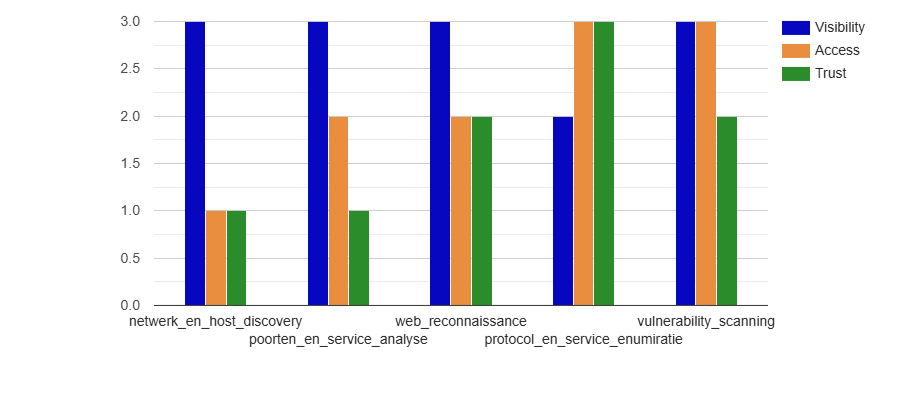
\includegraphics[width=\linewidth]{RAV_vergelijking_manueel_BarChart.png}
\caption{RAV vergelijking per tool van de manuele reconnaissance}
\label{fig:rav_barplot_manueel}
\end{figure}


Deze RAV-scores toont aan dat geen enkele tool over de drie secties uitsteekt.
\textit{Protocol en service enumeratie} geeft de meest gebalanceerde resultaten, met hoge scores voor access en trust, maar een lagere visibility, dit suggereert dat deze sectie zeer gedetailleerd is, maar minder zichtbare informatie kan verzamelen.
\textit{Netwerk en host discovery}, \textit{poorten en service analyse} en \textit{scoren hoog & Web reconnaissance} scoren hoog voor visibility, maar wisselend op access en trust. Dit reflecteert hun focus, het identificeren van hosts, poorten en services.
\textit{Vulnerability scanning} toont hoge scores voor visibility en acces, maar een lagere trust score.
Deze resultaten zijn verkregen door gekende commando's te gebruiken, de uitkomsten te evalueren en op basis hiervan vervolgcommando's te bepalen of op te zoeken.

Dit iteratieve proces verklaart waarom de uitvoeringstijd hier twee tot drie dagen bedraagt.
De tijd voor installatie en troubleshooting (niet-werkende commando's, alternatieven bedenken) wordt niet meegenomen in de uitvoeringstijd.
% Ook moet er gemeld worden dat de tijd dat genoemen werdt om geen valiede comanando's te laten uitvoeren en bedenken hier niet in de uitvoeringstijd is meegerekend.


\section{Automatisatie reconnaissance}

De automatisatie van de reconnaissancefase is uitgevoerd met behulp van zeven verschillende tools.
Deze tools verzamelen verschillende taken als scanning, service enumeratie en vulnerability mapping in een herhaalbare workflow.
Ook al zijn deze tools krachtig, is niet iedere tool geschikt voor een gecontroleerde omgeving zonder toegang tot het internet.
De tools die internet nodig hebben voor OSINT taken uit te voeren, zoals Shodan, Spiderfoot, Amass en Recon-ng, zijn uitgesloten van de volledige analyse, maar worden wel erkend voor de volledigheid.

Iedere tool is individueel en vergelijkend onderzocht, gebaseerd op hun technische gedrag, de output kwaliteit en betrouwbaarheid. Alsook op hun Uitvoeringstijd en de OSSTMM RAV-score.

Enkel de tools die volledig kunnen werken binnen in een lokaal netwerk zijn gebruikt.
Iedere tool werd geconfigureerd om de metasploitable2 te scannen, dit met de standaard of lichtelijke aanpassingen.
Alle data was verzameld voor de vergelijkende studie en een RAV-score.

\subsection{AutoRecon}
AutoRecon is een multi threaded enumeratie tool die een grote variatie heeft aan onderliggende scanning tools als Nmap, Feroxbuster, Nikto en meer.
Het detecteert automatisch open poorten, enumereert gelinkte services en verzameld relevante banners en metadata~\autocite{AutoRecon}. 
AutoRecon was getest in meerdere configuraties, waaronder de single-target en full-port scans 

% Deze tool past de flow van de scan af aan de voorafgaande scans en op basis hiervan verdere stappen ondernemen . 
% Hier integreert AutoRecon tools als Nmap, Feroxbuster, Nikto en meer voor een volledige reconnaissance scan.

\begin{itemize}
  \item \textbf{Sterktes:} hoge aanpasbaarheid, diepe integratie van meerdere tool, gestructureerde rapportering.
  \item \textbf{Limitaties:} relatieve hoge uitvoeringstijd veroorzaakt door de uitgebreide scanning.
  \item \textbf{Uitvoeringstijd:} ~78 minuten.
  \item \textbf{RAV-score:}
    {\small
    \begin{itemize}
      \item \textbf{Visibility:} hoog, haalde succesvol meerdere open poorten en service details. 
      \item \textbf{Access:} medium, capabel om de applicatie laag binnen te gaan en de specifieke service fingerprints te identificeren. 
      \item \textbf{Trust:} laag, geeft merendeel publieke informatie zonder gevoelige credentials en bestanden bloot te leggen. 
    \end{itemize}
    } 
\end{itemize}
\newpage

\subsection{CyberScan}

CyberScan is een snelle en lichte scanner ontworpen om open poorten en services te identificeren. 
De voornaamste rol is de snelle enumeratie om de host-beschikbaarheid en basis services te detecteren \autocite{Cyberscan}.

\begin{itemize}
  \item \textbf{Sterktes:} zeer snel, efficiënt voor een eerste verkenning.
  \item \textbf{Limitaties:} mist diepte in de scans en heeft geen vulnerability detectie.
  \item \textbf{Uitvoeringstijd:} ~5 minuten.
  \item \textbf{RAV-score:}
    \small{
    \begin{itemize}
      \item \textbf{Visibility:} medium, basis poort en protocol detectie.
      \item \textbf{Access:} laag, heeft geen service fingerprinting of vulnerablility scanning gedaan.
      \item \textbf{Trust:} geen, de output bevat geen gevoelige informatie. 
    \end{itemize}
    }
\end{itemize}

\subsection{Sn1per}
Sn1per is een volledig offensieve security scanner dat de reconnaissance aanvult met vulnerablility scanning en rapportage. 
Deze tool presteerde gelijkaardig met AutoRecon, maar geeft ook een gelimiteerde vulnerability analyse zoals standaard credential controles en openstaande admin interfaces \autocite{sn1per}.

\begin{itemize}
  \item \textbf{Sterktes:} rijke features, gecombineerd met meerdere scanning fases in één uitvoer.
  \item \textbf{Limitaties:} hoger systeem verbruik.
  \item \textbf{Uitvoeringstijd:} ~68 minuten.
  \item \textbf{RAV-score:}
    \small{
    \begin{itemize}
      \item \textbf{Visibility:} hoog, gedetailleerde outputs aan poorten, services en http endpoints.
      \item \textbf{Access:} medium, heeft een standaard vulnerability controle.
      \item \textbf{Trust:} medium, sommige zwakke configuraties en standaard instellingen waren blootgelegd.
    \end{itemize}
    }
\end{itemize}


\subsection{RustScan}

RustScan is geoptimaliseerd voor snelle poortscan's. 
Deze tool voert geen service enumeratie uit als standaard, maar kan in samenwerking met Nmap werken \autocite{RustScan}. 

\begin{itemize}
  \item \textbf{Sterktes:} buitengewone performatie, ideaal voor het scannen van grote IP-ranges.
  \item \textbf{Limitaties:} heeft toegevoegde tools nodig voor de volledige functionaliteit. 
  \item \textbf{Uitvoeringstijd:} minder dan 1 minuut.
  \item \textbf{RAV-score:}
    \small{
    \begin{itemize}
      \item \textbf{Visibility:} hoog, deedt een complete poortscan in slechts enkele seconden.
      \item \textbf{Access:} laag, staat niet in contact met services. 
      \item \textbf{Trust:} geen, heeft geen contact met services.
    \end{itemize}
    }
\end{itemize}

\subsection{Nuclei}
Nuclei is een template gebaseerde scanner, gebruikt om problemen zoals open panelen, misconfiguraite en verouderde software componenten te vinden \autocite{Nuclei}.

\begin{itemize}
  \item \textbf{Sterktes:} precisie scanning gebruik makende van community voorbeelden en makkelijk aanpasbaar.
  \item \textbf{Limitaties:} niet geschikt voor standalone gebruik in reconnaissance.
  \item \textbf{Uitvoeringstijd:} ~3 minuten.
  \item \textbf{RAV-score:}
    \small{
    \begin{itemize}
      \item \textbf{Visibility:} laag, afhankelijk van een eerder gekende enumeratie voor input. 
      \item \textbf{Access:} medium, identificeert gekende kwetsbaarheden gebaseerd op de analyse.
      \item \textbf{Trust:} hoog, capabel om verschillende misconfiguraties en gevoelige endpoints weer te geven.
    \end{itemize}
    }
\end{itemize}

\subsection{LazyRecon}
LazyRecon is gemaakt om de reconnaissance makkelijker te maken door tools samen te zetten in een geautomatiseerd script. 
In een internet-gelimiteerde omgeving zijn de OSINT functionaliteiten uitgeschakeld, resulterende in een gelimiteerde capaciteit \autocite{lazyrecon}.

\begin{itemize}
  \item \textbf{Sterktes:} simpele interface, geïntegreerd met meerdere tools.
  \item \textbf{Limitaties:} sterk vertrouwen in online bronnen, de offline functionaliteit is beperkt. 
  \item \textbf{Uitvoeringstijd:} ~9 minuten.
  \item \textbf{RAV-score:}
    \small{
    \begin{itemize}
      \item \textbf{Visibility:} medium, interne scan modules identificeren sommige lokale services en web applicaties.
      \item \textbf{Access:} laag, geen mogelijkheid om meer geavanceerdere scans te doen door de offline status.
      \item \textbf{Trust:} geen, geen gevoelige data gedetecteerd. 
    \end{itemize}
    }
\end{itemize}

\subsection{ReconFTW}

ReconFTW is een geavanceerde automatisatietool gemaakt voor een volledige reconnaissance. Net zoals LazyRecon zijn veel van de de functionaliteiten OSINT gebaseerd. 
In de offline mode geeft het nog steeds bruikbare scans binnenin het interne netwerk \autocite{reconftw}.

\begin{itemize}
  \item \textbf{Sterktes:} groote functionaliteit bij internet-gebaseerde enumeratie.
  \item \textbf{Limitaties:} grote limitatie offline.
  \item \textbf{Uitvoeringstijd:} ~14 minuten.
  \item \textbf{RAV-score:} 
    \small{
    \begin{itemize}
      \item \textbf{Visibility:} medium, onderzoekt toegangbare services en pagina's.
      \item \textbf{Access:} laag, verminderd door een niet internet-gebaseerde enumeratie.
      \item \textbf{Trust:} laag, minimale, gevoelige informatie achterhaald. 
    \end{itemize}
    }
\end{itemize}

\section{Resultatenanalyse geautomatiseerde reconnaissance}

De evaluatie van de tools is gebaseerd op hun betrouwbaarheid, uitvoeringstijd, bruikbaarheid, het CPU-gebruik en de RAV-score. 
In dit deel wordt analyse ondersteund door een staafdiagram die de RAV-scores voor elke tool visualiseert.  

\begin{figure}[H] 
\centering
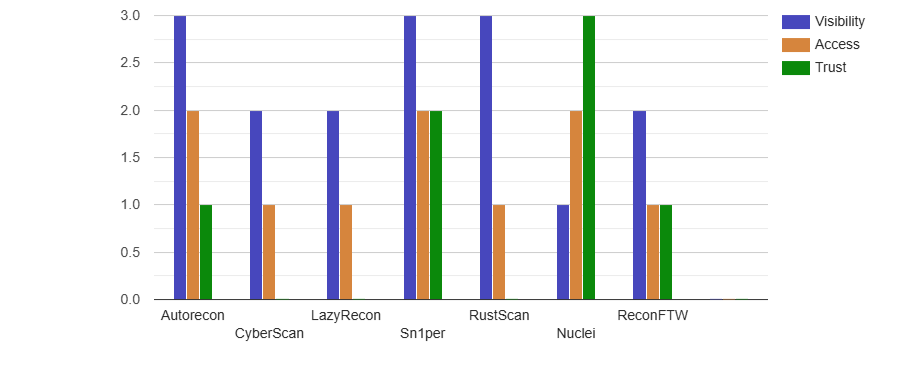
\includegraphics[width=\linewidth]{RAV_vergelijking_geautomatiseerd_BarChart.png}
\caption{RAV vergelijking per tool van de geautomatiseerde reconnaisansse}
\label{fig:rav_barplot_automatisatie}
\end{figure}

Deze RAV-score vergelijking laat zien dat geen enkele tool over al de drie secties uitsteekt. 
AutoRecon en Sn1per geven de meest gebalanceerde resultaten, met een hoge visibility en een gemiddelde access. Deze goede resultaten komen ten koste van een langere uitvoeringstijd.
Rustscan is onovertroffen in snelheid en poort scan's, terwijl Nuclei uitsteekt met zijn vulnerability detectie.
CyberScan en LazyRecon zijn op hun beurt ook geschikt voor snelle scans en ReconFTW, ondanks de offline-modus zijn ze nog steeds in staat bruikbare informatie te geven. 

Uit deze resultaten is af te leiden dat de automatisatie binnen de reconnaissance fase de efficiëntie verbetert. 
Iedere automatisatie tool die in deze vergelijking aan bod is gekomen heeft zijn eigen use case, wat op zijn beurt dan weer speelt met de effectiviteit van de tools.
Voor deze studie, met de focus op de reconnaissance fase en het zoveel mogelijk verzamelen van data, zijn de AutoRecon en Sn1per de meest bruikbare tools door hun uitgebreide analyse.

\section{Vergelijking van manueel en geautomatiseerde reconnaissance}
De manuele en de automatisatie reconnaissance zijn vergeleken op basis van betrouwbaarheid, Uitvoeringstijd, bruikbaarheid en de RAV-score.
\subsection{Betroubaarheid}

\begin{itemize}
  \item \textbf{manuele reconnaissance} de manuele reconnaissance is betrouwbaar voor lichtere commando's, maar is kwetsbaar voor foutmeldingen in complexere commando's. De menselijke interpretatie van de output is essentieel ter volledigheid, maar geeft ook een variabiliteit in de resultaten.
  \item \textbf{automatisatie reconnaissance} 
  \begin{itemize}
    \item \textbf{AutoRecon, Sn1per, LazyRecon, RustScan, } Zeer betrouwbaar (90-95\%), occasionele errors met web scans.
    \item \textbf{CyberScan} Redelijk betrouwbaar (85\%) door veroudering en simpliciteit, niet zo consistent.
    \item \textbf{Nuclei, ReconFTW} Redelijk betrouwbaar (50\%) niet veel mogelijkheden door de offline status.
  \end{itemize}
  \item \textbf{conclusie} De manuele aanpak is beter voor gedetailleerde scans, maar is meer onderhevig aan fouten. De automatisatietools zijn betrouwbaarder, maar kunnen de diepgang van de manuele testen niet vervangen.
\end{itemize}

\subsection{Uitvoeringstijd}

\begin{itemize}
  \item \textbf{Manuele reconnaissance} twee tot drie dagen voor de volledige reconnaissancefase. Als dit uitgevoerd wordt door het bash script kan dit verminderen naar ~30 minuten. Echter vertelt dit niet het hele verhaal van de uitvoeringstijd, het merendeel van de tijd gaat naar het verstaan en interpreteren van de output en deze analyseren voor een vervolgcommando.
  \newpage
  \item \textbf{Automatisatie reconnaissance} 
  \begin{itemize}
    \item \textbf{CyberScan, RustScan} 5-60 seconden
    \item \textbf{Nuclei} 5-20 minuten
    \item \textbf{AutoRecon} 15-30 minuten
    \item \textbf{ReconFTW, LazyRecon} 15-60 minuten
    \item \textbf{Sn1per} 1-120 minuten
  \end{itemize}
  \item \textbf{conclusie} De automatisatie tools zijn aanzienlijk sneller in uitvoeringstijd dan de manuele reconnaissance, echter is dit niet volledig door de tijd die in beslag wordt genomen voor installatie en configuratie van de tools.
\end{itemize}


\subsection{Bruikbaarheid}
\begin{itemize}
  \item \textbf{Manuele reconnaissance} vereist een grote kennis van de tools en de output, dit kan een probleem zijn bij minder ervaren pentesters.
  \item \textbf{Mutomatisatie reconnaissance} 
  \begin{itemize}
    \item \textbf{AutoRecon, LazyRecon, Sn1per, LazyRecon, ReconFTW} gebruiksvriendelijk en eenvoudig te gebruiken, maar de output kan moeilijker verstaanbaar zijn.
    \item \textbf{CyberScan, Nuclei} enkele kennis van de tool vereist.
  \end{itemize}
  \item \textbf{conclusie} De automatisatietools zorgen ervoor dat de barrière voor de nodige kennis van de tools lager is.
\end{itemize}


\subsection{OSSTMM overeenkomst}
\begin{itemize}
  \item \textbf{Standaardiseren} De manuele aanpak is gestructureerd, maar is afhankelijk van de kennis van de pentester. AutoRecon en Sn1per hebben een makkelijke workflow en zijn gestructureerd.
  \item \textbf{Reproduceerbaar} De manuele aanpak is reproduceerbaar in een gecontroleerde omgeving, geautomatisatiseerde tools zorgen voor meer consistentie.
  \item \textbf{Neutraal} Bij de manuele aanpak zijn alle tools open source en daarvoor neutraal, de meeste tools bij de geautomatiseerde aanpak zijn ook open-source maar LazyRecon en reconFTW gebruiken hun eigen gegevens dat kan leiden tot een lichte bias.
  \item \textbf{Meetbare risico} de RAV-scores zorgen voor de meetbare risico's.
\end{itemize}



% \subsection{OSSTMM-Aligned Testing Protocol}

% \begin{itemize}
%   \item \textbf{Pre-Test fase}:
%   \begin{itemize}
%     \item defineer de Rules of Engagement (RoE) voor iedere tool.
%     \item geef securiy best practices aan.
%     \item configureer de testomgeving.
%   \end{itemize}
  
%   \item \textbf{Test Execution}:
%   \begin{itemize}
%     \item test de tool tegen Metasploitable 2.
%     \item documenteer iedere stap van de configuratie. 
%     \item documenteeer de systeem 
%     \item Monitored systeem gegevens (CPU, memory, netwerk)
%   \end{itemize}
  
%   \item \textbf{Post-Test analyse}:
%   \begin{itemize}
%     \item verzamel outputs en logs van de tools.
%     \item analyseer de resultaten.
%     \item berken de RAV score.
%   \end{itemize}
% \end{itemize}

% \section{tool evaluatie}

% \subsection{Network Scanning Suite}

% \subsubsection{Nmap Advanced Features}
% \begin{itemize}
%   \item \textbf{Scripting Engine}:
%   \begin{itemize}
%     \item 600+ NSE scripts categorized by:
%     \begin{itemize}
%       \item Discovery (35\%)
%       \item Vulnerability (25\%)
%       \item Exploit (15\%)
%       \item Miscellaneous (25\%)
%     \end{itemize}
%   \end{itemize}
  
%   \item \textbf{Performance Optimization}:
%   \begin{itemize}
%     \item Timing templates (-T0 to -T5)
%     \item Parallel scan algorithms
%     \item Adaptive host discovery
%   \end{itemize}
% \end{itemize}

% \begin{minted}[linenos,breaklines,frame=single]{bash}
% nmap -sV -sC -p- -T4 \
%      -oA scan_results \
%      target_ip
% \end{minted}






% %%=============================================================================
%% Literatuurstudie
%%=============================================================================

\chapter{\IfLanguageName{dutch}{Literatuurstudie}{Literatuurstudie}}
\label{ch:Literatuurstudie}

\section{Inleiding tot Penetratietesten}
Penetratietesten (pentests) zijn cyberaanvallen, uitgevoerd door ethische hackers in een gecontroleerde simulatie om uit de netwerken, systemen of applicaties kwetsbaarheden te halen voordat ongeautoriseerde actoren deze kwetsbaarheden kunnen gebruiken \textcite{Shebli}. 
Deze testen zijn cruciaal voor een organisatie om beveiligingsrisico's uit de systemen te halen en om aan de veiligheidsnormen te voldoen (bv. GDPR, ISO 27001), ook om vertrouwen bij de klanten te winnen \parencite{Dalalana2017}.

\subsection{Types Penetratietesten}
Pentests zijn vaak niet eenzijdig, deze pentesten worden op verschillende manieren gebruik, voor verschillende doelen, targets en specifieke objecten.
Hiervoor zijn er verschillende pentest strategieën deze kun je kiezen op basis van welke specifieke objectieven die je wilt aanhalen \textcite{Vats2020} bespreekt er een paar:\sloppy

\begin{itemize}
    \item Externe testen
    \item Interne testen
    \item Blinde testen
    \item Dubbel blinde testen
    \item Gerichte testen
\end{itemize}

Daarnaast zijn er verschillende soorten testen die organisaties kunnen uitvoeren, waarbij de keuze tussen deze methoden afhankelijk is van de scope en vereisten van een organisatie:

\begin{itemize}
    \item \textbf{Black box testing:} De tester heeft geen informatie of voorkennis van het systeem, vergelijkbaar met een externe aanval
    \item \textbf{White box testing:} De tester krijgt volledige toegang tot de netwerkarchitectuur en broncode
    \item \textbf{Gray box testing:} De tester krijgt beperkte gegevens, bijvoorbeeld inloggegevens voor low-privilege accounts
\end{itemize}
\autocite{Khamdamovich2021}

\section{Noodzaak van Pentests}
Zonder pentesten kunnen bedrijven verschillende risico's oplopen:

\begin{itemize}
    \item \textbf{Financiële schade:} volgens IBM kan een data lek een bedrijf €4,88 miljoen kosten inclusief boetes en herstelkosten \autocite{IBM2023}
    \item \textbf{Operationele downtime:} vele aanvallen lijden tot een gemiddelde van 21 dagen downtime \autocite{DBIR2023}
    \item \textbf{Reputatie schade:} Een publiekelijk geweten cyberaanval kan ervoor zorgen dat een bedrijf 60\% van zijn klanten verliest \autocite{Ponemon2022}
\end{itemize}

\section{De Reconnaissance-Fase}
Ieder type pentest begint met een reconnaissance-fase, de kritieke eerste stap waar de kern informatie verzamelen is. 
Deze fase omvat het verzamelen van informatie over het doelwit om zwakke punten te identificeren. 
Zoals \textcite{Shah} zegt ``Zonder grondige reconnaissance is een pentest gedoemd om oppervlakkige resultaten te behalen.''
Dit proces legt de basis voor de volgende stappen in de pentest \autocite{Kothia}.

De term Reconnaissance vindt zijn oorsprong in het Frans (1800 - 1810) en betekent letterlijk verkennen. 
Dit concept ontstond vanuit de militaire strategie, waar de Calvarie eenheden probeerden waardevolle informatie te verzamelen over het terrein en de vijand, zodat ze met deze informatie een effectieve aanval konden plannen.
Deze oude principes vertalen zich vandaag naar de cybersecurity, waar het draait om kwetsbaarheden te identificeren voordat een aanval zich kan plaatsvinden.
Historisch gezien was Reconnaissance een taak van de cavalerie. Zij gebruikten vele manieren om informatie te verzamelen zoals visuele observaties, verkenningstochten en zelfs vroege vormen van social engineering. 
Deze informatie vormde de basis voor het plannen van een aanvallen en in te spelen op de zwaktes van de vijand.
In de moderne cybersecurity wereld volgt reconnaissance nog steeds dezelfde principes maar dan digitaal, zoals gevoelige documenten, netwerken en social engineering gebruiken om kwetsbaarheden binnen het bedrijf te vinden.

\subsection{Variaties binnen de Reconnaissance-Fase}
De reconnaissance kunnen we opsplitsen in een passieve en een actieve kant, elke met hun eigen methoden en tools. 
Bij passieve reconnaissance is het doel om informatie te verzamelen zonder dat er direct contact is tussen het doelwit en de pentester.
Hier zijn er verschillende technieken voor zoals de OSINT (Open Source Intelligence) dat gebruik maakt van publieke bronnen zoals databases, sociale media en forums \autocite{Dalalana2017}. 
Shodan maakt gebruik van scanning van IoT apparaten en poorten op toegankelijke internetverbindingen \autocite{Monero2025}.
Deze techniek heeft een zeer lage kans op detectie, maar dit beperkt de diepgang, Hiermee is er slechts 40\% van de kwetsbaarheden dat aan het licht komt \parencite{Mahin2014}.
Bij de actieve reconnaissance staat de pentester echter wel direct in contact met het doelwit om informatie te verkrijgen, hier bestaan ook vele technieken voor zoals een Portscanner die open poorten en services kan detecteren \autocite{Monero2025}. 
Vulnerability scanning is ook een techniek om automatisch bekende kwetsbaarheden te detecteren \autocite{GOEL2015}. 
Deze testen hebben wel een hogere nauwkeurigheid tot 92\% bij geavanceerde tools maar dit kan firewalls of IPS systemen activeren \parencite{Li2022}.

\subsection{Automatisering}
Automatisatie maakt het mogelijk om de reconnaissance fase te versnellen. 
\textcite{Hoang} heeft deep reinforcement learning (RL) gebruikt voor de geautomatiseerde aanpak voor pentesten. 
Dit model is gebaseerd op het A3C-algoritme. Dit algoritme leert om op zichzelf beslissingen te nemen, deze beslissingen kunnen gaan over het kiezen van de payloads en het gebruiken van de juiste exploits. 
Zijn methode is gericht op drie functies: informatie verzamelen, exploitatie en rapportage \autocite{Hoang}.
Zoals \textcite{Kothia} beschrijft, kan de eerste fase binnen pentesting in de reconnaissance-fase veel efficiënter gebeuren met behulp van automatisatie. 
Er zijn veel open source tools beschikbaar, maar helaas vraagt het gebruik van deze tools nog veel handmatige inspanning om ze te integreren.
Er is een geautomatiseerde aanpak gecreëerd door Kothia om deze tools efficiënter te integreren. 
Deze resultaten toonden aan dat dit implementatie tijd kan besparen en zorgt voor een betere nauwkeurige uitvoering \parencite{Kothia}.

\subsection{Innovaties in Reconnaissance}
Om pentests te automatiseren, zijn er verschillende tools beschikbaar om efficiënt en snel informatie te verzamelen. 
Onder andere AutoRecon, Cyberscan, Sn1per, RustScan, Nuclei, LazyRecon en ReconFTW deze tools zijn vaak open source en zijn krachtige tools ontwikkeld om het proces van reconnaissance te versnellen \autocite{Shebli}.

\section{Vergelijkingen}
Automatisering kan de efficiëntie en snelheid van de reconnaissance-fase verhogen. Er zijn veel tools die snel een netwerk kunnen scannen en de kwetsbaarheden kunnen detecteren. 
Door automatisatie kunnen organisaties sneller en kosteneffectieve tests uitvoeren. Deze automatisatie kan echter wel leiden tot een kwaliteitsverlies, d.w.z. dat het systeem mogelijks niet alle kwetsbaarheden vindt \parencite{peris}. 
Meer diepgaande Scans gebeuren vaak handmatig, deze zijn flexibeler dan een geautomatiseerde test. Met de handmatige aanpak kun je makkelijker complexe kwetsbaarheden terugvinden die niet makkelijk te detecteren vallen bij een geautomatiseerde tool \parencite{techtarget2023}. 
Het kiezen tussen een handmatige of een geautomatiseerde pentest komt vaak voor, deze keuze hangt af van de specifieke vereisten van de organisatie. \textcite{Monero2025} analyseerde telkens 50 cases studies waar er een geautomatiseerde en een hybride aanpak kwetsbaarheden detecteerde, waar de studie een hybride aanpak nam konden ze in deze testcase 85\% van de kwetsbaarheden detecteren, tegenover de 70\% bij volledige automatisering.
Bij een voorbeeld van \parencite{Whitaker2005}, waar simulaties aantonen dat onvoldoende training in het gebruik van tools kan leiden tot 25\% vals positieve resultaten.
Dit benadrukt de gestandaardiseerde protocollen, zoals het OSSTMM framework om dit tegen te gaan en consistentie te garanderen.

\section{Efficiëntie en uitdagingen}
Momenteel zijn er nog enkele uitdagingen bij pentests; zoals \textcite{Fugkeaw} beschrijft, dat er nog te veel vertrouwen is in de experten van het vak bij het beoordelen van de al dan niet geautomatiseerde reconnaissance-fase. Bij veel methoden is er nog vaak de verwachting dat er een menselijke input nodig is bij het maken van een vulnerability assessment (VA) bij het analyseren en prioriteren. Dit verhoogt de kans op menselijke fouten en is tijdintensief, ook zijn de testen vaak inconsistent door de individuele voorkeuren van de pentester \parencite{Ghanem}. Binnen pentesting ontdekken en gebruiken professionals vaak nieuwe technologieën, één van deze nieuwe technologieën is het gebruik van kunstmatige intelligentie. Zoals het Intelligent Automated Penetration Testing System (IAPTS), dat ontwikkeld is door \textcite{Ghanem}, in deze studie is er gebruik gemaakt van reinforcement learning (RL) om testpatronen te leren en te optimaliseren. Als we deze technologie gebruiken in de reconnaissance-fase samen met het wiskundige model om beslissingen te nemen, de Partially observed Markov decision proces (POMDP), kunnen we nauwkeurigere resultaten zien. Echter blijft het belangrijk dat er een juiste balans zit tussen automatisatie en menselijke controle. Menselijke testers hebben vaker meer creativiteit en intuïtie, wat moeilijk is te vervangen door een geautomatiseerde tool. Daarom is het belangrijk onderzoek te blijven uitvoeren naar hybride modellen.






% Voeg hier je eigen hoofdstukken toe die de ``corpus'' van je bachelorproef
% vormen. De structuur en titels hangen af van je eigen onderzoek. Je kan bv.
% elke fase in je onderzoek in een apart hoofdstuk bespreken.

%\input{...}
%\input{...}
%...

%%=============================================================================
%% Conclusie
%%=============================================================================

\chapter{Conclusie}%
\label{ch:conclusie}

% TODO: Trek een duidelijke conclusie, in de vorm van een antwoord op de
% onderzoeksvra(a)g(en). Wat was jouw bijdrage aan het onderzoeksdomein en
% hoe biedt dit meerwaarde aan het vakgebied/doelgroep? 
% Reflecteer kritisch over het resultaat. In Engelse teksten wordt deze sectie
% ``Discussion'' genoemd. Had je deze uitkomst verwacht? Zijn er zaken die nog
% niet duidelijk zijn?
% Heeft het onderzoek geleid tot nieuwe vragen die uitnodigen tot verder 
%onderzoek?

De resultaten van dit onderzoek hebben kunnen aantonen dat een geautomatiseerde aanpak van de reconnaissance fase de efficiëntie aanzienlijk kan verhogen.
Waar tools als RustScan volledige scans kunnen voltooien in minder dan een minuut, gaven AutoRecon en Sn1per een uitgebreide evaluatie van resultaten, in een langere uitvoeringstijd (~79 tot 129 minuten).
Cyberscan en Nuclei waren efficiënt voor een relatief snelle verkenning en vulnerability detectie, waar Layzyrecon en ReconFTW beperkter waren door de offline omgeving.
Deze konden door hun manuele aanpak een diepere verkenning uitvoeren, weliswaar ten kostte van de uitvoeringstijd.
Belangrijk te melden is dat de tijd van de manuele aanpak (twee tot drie dagen, ~30 minuten met bash script) enkel maar de actieve verwerkingstijd omvat.
Het analyseren van de commando's en het onderzoeken naar volgcommando's vraagt tijd, wat de algemene tijd van de manuele methode aanzienlijk vergroot.
Bovendien is de tijd van de installatie van de tools, de gefaalde tools en commando's niet meegerekend in dit rapport.
Een combinatie van de tool RustScan, voor snelheid, en Sn1per, voor de diepgang bleek het meest effectief te zijn volgens het OSSTMM Framework.
Een kritische beoordeling van de resultaten bevestigt de verwachtingen dat dat automatisatie de uitvoeringstijd en consistentie verbetert, maar dat de manuele aanpak beter is voor diepgaande analyses. Al was het verschil meer aanwezig dan oorspronkelijk gedacht.
De tijd van het analyseren en bedenken van een vervolgcommando speelde een grotere factor dan initieel gedacht.
Deze studie heeft ook nieuwe vragen naarboven gehaald zoals, hoe automatische tools werken op dynamische netwerken, of hybride aanpakken verder kunnen worden geoptimaliseerd en hoe mislukte commando's kunnen worden onderzocht om de workflow te verbeteren?
Deze vragen kunnen in een toekomstig onderzoeken worden beantwoord. 
Daarnaast vormt de toepassing van machine learning voor intelligente toolselectie een veelbelovende onderzoeksrichting, gezien het potentieel om de automatische reconnaisansse verder te optimaliseren.

% Bovendien verdient de toepassing van machine-learning voor Intelligente tool selectie is een intersante een nader onderzoek.
% Daarnaast vormt de toepassing van machine-learning voor Intelligente tool selectie is een veelbelovende onderzoeksrichting.

% Een bijzonder interessant pad naar de implementatie van machine learning-algoritmen voor geautomatiseerde selectie van security tools blijft open staan.
%  betreft de vraag van machine-learning voor Intelligente tool selectie, wat naar deverwachtingen de efficiëntie aanzienlijk zou verhogen.
% betreft de implementatie van machine learning-algoritmen voor geautomatiseerde selectie van security tools


% Daarnaast vormt de toepassing van machine-learning voor Intelligente tool selectie is een intersante onderzoeksrichting.

%---------- Bijlagen -----------------------------------------------------------

\appendix

\chapter{Onderzoeksvoorstel}

Het onderwerp van deze bachelorproef is gebaseerd op een onderzoeksvoorstel dat vooraf werd beoordeeld door de promotor. Dat voorstel is opgenomen in deze bijlage.

%% TODO: 
%\section*{Samenvatting}

% Kopieer en plak hier de samenvatting (abstract) van je onderzoeksvoorstel.

% Verwijzing naar het bestand met de inhoud van het onderzoeksvoorstel
%---------- Inleiding ---------------------------------------------------------

% TODO: Is dit voorstel gebaseerd op een paper van Research Methods die je
% vorig jaar hebt ingediend? Heb je daarbij eventueel samengewerkt met een
% andere student?
% Zo ja, haal dan de tekst hieronder uit commentaar en pas aan.

%\paragraph{Opmerking}

% Dit voorstel is gebaseerd op het onderzoeksvoorstel dat werd geschreven in het
% kader van het vak Research Methods dat ik (vorig/dit) academiejaar heb
% uitgewerkt (met medesturent VOORNAAM NAAM als mede-auteur).
% 




\section{Inleiding}%
\label{sec:inleiding}

Penetratietests(pentests) hebben een cruciale rol bij cybersecurity, waarbij cybersecurity en IT-professionals proberen in te breken in het intern netwerk 
van een organisatie of bedrijf om toegang te krijgen tot het systeem, dit om te voorkomen dat er black hat hackers toegang kunnen krijgen tot hun systeem. 
De eerste fase binnen dit proces in de reconnaissance-fase, waar er zo veel mogelijk data wordt verzameld over het doelwit. Dit is één van de belangrijkste fases, 
aangezien deze fase de basis legt voor rest van de pentest. Als deze fase handmatig wordt uitgevoerd zal deze stap te veel tijd kosten. 
%Met efficiëntie als doel zoekt dit onderzoek naar geautomatiseerde tools om het handmatige te vervangen.
het doel is om efficiëntie te bereiken door het vinden van geautomatiseerde tools om het handmatige proces te vervangen.
Het onderzoek richt zich op het vergelijken van de beschikbare tools en technieken om er de meest efficiënte tool of framework uit te halen, weliswaar zonder kwaliteitsverlies van de verzamelde informatie.
De belangerijkste doelgroep waar mijn studie op richt zijn IT’ers die werken met pentests, zoals cybersecurity- en IT-professionals en bedrijven die regelmatig hun systemen testen op kwetsbaarheden. 
Deze doelgroep is op zoek naar een betrouwbare tool dat efficiënt is en een snelle werking heeft. 
%Deze literatuuronderzoek heeft betrekking op o.a.
Om dit te analyseren zal ik een literatuuronderzoek doen naar enkele bestaande tools waaronder 
AutoRecon, Recon-ng en Shodan, aangevuld met testen op pentest scenario’s om deze werking te analyseren en hun efficiëntie te vergelijken. 
Het eindresultaat van dit onderzoek zal bestaan uit aanbevelingen voor de intigratie en werking van deze tools.


% Waarover zal je bachelorproef gaan? Introduceer het thema en zorg dat volgende zaken zeker duidelijk aanwezig zijn:

% \begin{itemize}
%   \item kaderen thema
%   \item de doelgroep
%   \item de probleemstelling en (centrale) onderzoeksvraag
%   \item de onderzoeksdoelstelling
% \end{itemize}

% Denk er aan: een typische bachelorproef is \textit{toegepast onderzoek}, wat betekent dat je start vanuit een concrete probleemsituatie in bedrijfscontext, een \textbf{casus}. Het is belangrijk om je onderwerp goed af te bakenen: je gaat voor die \textit{ene specifieke probleemsituatie} op zoek naar een goede oplossing, op basis van de huidige kennis in het vakgebied.

% De doelgroep moet ook concreet en duidelijk zijn, dus geen algemene of vaag gedefinieerde groepen zoals \emph{bedrijven}, \emph{developers}, \emph{Vlamingen}, enz. Je richt je in elk geval op it-professionals, een bachelorproef is geen populariserende tekst. Eén specifiek bedrijf (die te maken hebben met een concrete probleemsituatie) is dus beter dan \emph{bedrijven} in het algemeen.

% Formuleer duidelijk de onderzoeksvraag! De begeleiders lezen nog steeds te veel voorstellen waarin we geen onderzoeksvraag terugvinden.

% Schrijf ook iets over de doelstelling. Wat zie je als het concrete eindresultaat van je onderzoek, naast de uitgeschreven scriptie? Is het een proof-of-concept, een rapport met aanbevelingen, \ldots Met welk eindresultaat kan je je bachelorproef als een succes beschouwen?



%---------- Stand van zaken ---------------------------------------------------

\section{Literatuurstudie}%
\label{sec:literatuurstudie}

\subsection{Reconnaissance in penetratietests}

De reconnaissance-fase, of de verkenningsfase, is een fase binnen pentests die een cruciale rol heeft, maar vaak ook de meest tijdrovende stap, 
het kan weken tot maanden duren, afhankelijk van de complexiteit van het target en de technieken die worden gebruikt~\autocite{Shah}. 

Het doel van de reconnaissance-fase binnen pentests is het creëren van een volledig beeld om de 
kwetsbaarheden van het doelwit bloot te leggen. Dit process legt de basis voor de
volgende stappen in de pentest \autocite{Kothia}.

Tijdens deze fase maken testers of aanvallers gebruik van actieve en passieve technieken om zoveel
mogelijk informatie verzamelen. De passieve methode houdt in dat er informatie over het doelwit wordt verzameld zonder dat er direct contact mee wordt gemaakt, 
de actieve methode is wel direct verbonden met het doelwit, bijvoorbeeld door gebruik te maken van tools zoals Nmap, om open poorten te detecteren~\autocite{Shah}.


\subsection{Automatisering}

~\textcite{Hoang} heeft een geautomatiseerde aanpak voor pentesten waarin hij deep reinforcement 
learning (RL) gebruikt. Zijn model is gebaseerd op het A3C-algoritme. Dit algoritme leert zichzelf de geschikte acties aan, dit kan 
gaan over het kiezen van de payloads en het benutten van de juiste kwetsbaarheden. Zijn methode is gericht op drie functies: informatie verzamelen, 
exploitatie en rapportage. Hoang toont daarmee aan dat het gebruik van deze aanpak niet enkel de prestatie verbetert, maar ook dat het systeem de resultaten 
kan opslaan om die toe te passen op nieuwe situaties.~\autocite{Hoang}.


Volgens ~\textcite{Kothia} kan de eerste fase binnen pentesting in reconnaissance-fase veel 
efficiënter gebeuren met behulp van automatisatie. Er zijn veel open source tools beschikbaar, maar helaas vraagt het gebruik van deze 
tools nog veel handmatige inspanning om ze te integreren. Kothia heeft een geautomatiseerde aanpak gecreëerd om deze tools
efficiënter te integreren. De resultaten van de studie toonde aan dat deze implementatie, tijd 
bespaarde en zorgde voor een betere en nauwkeurigere uitvoering~\autocite{Kothia}.


\newline \subsection{Tools en Frameworks}
\newline Om pentests te automatiseren, zijn er verschillende frameworks en tools beschikbaar om 
efficiënt en snel informatie te verzamelen. De meeste van deze tools zijn open source, waaronder 
AutoRecon, Recon-ng, Shodan en Nmap. Deze tools zijn ontwikkeld om robust te zijn en het process van de Reconnaissance-fase te versnellen ~\autocite{Shebli}.


\subsection{Vergelijkingen}

Automatisering kan de efficiëntie en snelheid van de reconnaisance-fase verhogen. Er zijn vele tools die snel een netwerk kunnen scannen, 
er de kwetsbaarheden uit kunnen halen en de kwetsbaarheden kunnen detecteren. Door automatisatie kunnen 
organisaties sneller en kosten-effectiever tests uitvoeren. Deze automatisatie kan echter wel leiden tot een kwaliteitsverlies, 
d.w.z. dat mogelijks het systeem niet alle kwetsbaarheden vindt. ~\autocite{peris}

Meer diepgaande scans worden vaak handmatig gedaan, deze zijn flexibeler dan een geautomatiseerde test. 
Met de handmatige aanpak kun je makkelijker complexe kwetsbaarheden terugvinden die niet makkelijk te detecteren vallen bij 
een geautomatiseerde tool.~\autocite{techtarget} 

Vaak wordt er een keuze gemaakt tussen een handmatige of een geautomatiseerde penettest, deze keuze hangt vaak af van de specifieke  
vereisten van de organisatie. Echter wordt er ook niet gekozen om puur handmatig of geautomatiseerde pentest te maken, maar wordt
een hybride model vaker gebruikt. Dit is vaak de ideale oplossing waarbij automatisatie en menselijke ervaring elkaar kunnen 
aanvullen voor een efficiënte Reconnaissance-fase ~\autocite{techtarget}.

\subsection{Efficiëntie en uitdagingen}

% Momenteel zijn er nog enkele uitdagingen bij pentests, zoals ~\textcite{Fugkeaw} beschrijft, dat er nog te veel wordt vertrouwd op de experten van het vak bij het beoordelen van de al dan niet geautomatiseerde Reconnaissance-fase.
% Bij vele methoden wordt er vaak nog op gerekend dat er een menselijke input is bij het maken van een vulnerability assessment (VA) bij het analyseren en prioriteren. Dit verhoogt de kans op menselijke fouten en is tijdintensief, ook zijn de testen vaak 
% inconsistent door de individuele voorkeuren van de pentester volgens ~\textcite{Ghanem}.
% Binnen pentesting worden er nog vaak nieuwe technologieën ontdekt en gebruikt, één van deze nieuwe technologieën is het gebruik van kunstmatige intelligentie. Zoals Het Intelligent Automated Penetration Testing System (IAPTS), ontwikkeld door \textcite{Ghanem}, 
% hier wordt er gebruik gemaakt van reinforcement learning (RL) om testpatronen te leren en te optimaliseren. Als we deze technologie gebruiken in de reconnaissance-fase samen met het wiskundige model om beslissingen te maken; de Partially observed Markov decision process (POMDP) 
% kunnen we nauwkeurigere resultaten behalen. 
% Echter blijft het belangrijk dat er een juiste balans zit tussen automatisatie en menselijke controle. Menselijke testers hebben vaker meer creativiteit en intuïtie wat moeilijk is te vervangen door een geautomatiseerde tool. Daarom blijft het belangrijk om te blijven onderzoeken naar hybride modelen.

Momenteel zijn er nog enkele uitdagingen bij pentests, zoals ~\textcite{Fugkeaw} beschrijft, dat er nog te veel wordt vertrouwd op de experten van het vak bij het beoordelen van de al dan niet geautomatiseerde Reconnaissance-fase.Bij vele methoden wordt er vaak nog op gerekend dat er een menselijke input is bij het maken van een vulnerability assessment (VA) bij het analyseren en prioriteren. Dit verhoogt de kans op menselijke fouten en is tijdintensief, ook zijn de testen vaakinconsistent door de individuele voorkeuren van de pentester volgens ~\textcite{Ghanem}.
Binnen pentesting worden er nog vaak nieuwe technologieën ontdekt en gebruikt, één van deze nieuwe technologieën is het gebruik van kunstmatige intelligentie. Zoals Het Intelligent Automated Penetration Testing System (IAPTS), ontwikkeld door \textcite{Ghanem},hier wordt er gebruik gemaakt van reinforcement learning (RL) om testpatronen te leren en te optimaliseren. Als we deze technologie gebruiken in de reconnaissance-fase samen met het wiskundige model om beslissingen te maken; de Partially observed Markov decision process (POMDP) kunnen we nauwkeurigere resultaten behalen. Echter blijft het belangrijk dat er een juiste balans zit tussen automatisatie en menselijke controle. Menselijke testers hebben vaker meer creativiteit en intuïtie wat moeilijk is te vervangen door een geautomatiseerde tool. Daarom blijft het belangrijk om te blijven onderzoeken naar hybride modelen.




% Hier beschrijf je de \emph{state-of-the-art} rondom je gekozen onderzoeksdomein, d.w.z.\ een inleidende, doorlopende tekst over het onderzoeksdomein van je bachelorproef. Je steunt daarbij heel sterk op de professionele \emph{vakliteratuur}, en niet zozeer op populariserende teksten voor een breed publiek. Wat is de huidige stand van zaken in dit domein, en wat zijn nog eventuele open vragen (die misschien de aanleiding waren tot je onderzoeksvraag!)?

% Je mag de titel van deze sectie ook aanpassen (literatuurstudie, stand van zaken, enz.). Zijn er al gelijkaardige onderzoeken gevoerd? Wat concluderen ze? Wat is het verschil met jouw onderzoek?

%Verwijs bij elke introductie van een term of bewering over het domein naar de vakliteratuur, bijvoorbeeld~\autocite{Hykes2013}! Denk zeker goed na welke werken je refereert en waarom.

% Draag zorg voor correcte literatuurverwijzingen! Een bronvermelding hoort thuis \emph{binnen} de zin waar je je op die bron baseert, dus niet er buiten! Maak meteen een verwijzing als je gebruik maakt van een bron. Doe dit dus \emph{niet} aan het einde van een lange paragraaf. Baseer nooit teveel aansluitende tekst op eenzelfde bron.

% Als je informatie over bronnen verzamelt in JabRef, zorg er dan voor dat alle nodige info aanwezig is om de bron terug te vinden (zoals uitvoerig besproken in de lessen Research Methods).

% Voor literatuurverwijzingen zijn er twee belangrijke commando's:
% \autocite{KEY} => (Auteur, jaartal) Gebruik dit als de naam van de auteur
%   geen onderdeel is van de zin.
% \textcite{KEY} => Auteur (jaartal)  Gebruik dit als de auteursnaam wel een
%   functie heeft in de zin (bv. ``Uit onderzoek door Doll & Hill (1954) bleek
%   ...'')

% Je mag deze sectie nog verder onderverdelen in subsecties als dit de structuur van de tekst kan verduidelijken.

%---------- Methodologie ------------------------------------------------------
\section{Methodologie}%
\label{sec:methodologie}

Een combinatie van methoden zullen worden gebruikt om de onderzoeksvraag te beantwoorden, er zal onder andere gebruik
gemaakt worden van de literatuurstudie, onderzoeken en vergelijkende analyses. Hieronder zijn de stappen beschreven:

\subsection{Literatuurstudie}

De literatuurstudie zal de basis vormen voor dit onderzoek. Door een grondige analyse te maken van de reeds bestaande tools en studies,
die gebruikt worden in de reconnaissance-fase van pentests, kan er een overzicht gemaakt worden van de huidige situatie.
hierbij wordt er rekening gehouden met de vindingen van~\textcite{Shah,Kothia} die de voordelen en beperkingen aantonen binnen de reconnaissance-fase.
Ook zal er rekening gehouden worden met nieuwe technologieën zoals die van ~\textcite{Ghanem,Hoang} waar er gebruikt wordt gemaakt van
reinforcement learning (RL), Intelligent Automated Penetration Testing System (IAPTS) en POMDP-modellen. De implementatie van bestaande
tools en frameworks zoals AutoRecon en Recon-ng zal ook onderzocht worden~\autocite{Shebli}.

De resultaten van deze literatuurstudie zal worden gebruikt om een kader te schetsen voor de verdere ontwikkeling van dit onderzoek.

\subsection{Experimenteel onderzoek}

Om de effectiviteit van de automatisering te kunnen demonstreren in de reconnaissance-fase zal er een Een Proof of Concept (PoC) opgestart worden.
Dit omvat dat er een workflow zal worden geïmplementeerd met behulp van de automatisatie tools waaronder AutoRecon en Recon-ng. Deze
Workflow zal getest worden op een gesimuleerd netwerk waar er bekende kwetsbaarheden op staan om via deze data de snelheid,
nauwkeurigheid en consistentie te meten. Met behulp van deze data kunnen we nieuwe technologieën integreren om onze automatisatie te optimaliseren
zoals reinforcement learning (RL) om patronen te herkennen.
Aan de hand van de verzamelde informatie zal het onderzoek geëvalueerd worden aan de hand van nauwkeurigheid, tijdswinst en consistentie.


%----------------------------------------------------------------------------------------------------------
\subsection{Meetbare Criteria voor Analyse}

Om de resutaten van de analyse te beoordelen zal er gewerkt worden met de volgende meetbare criteria:
- De nodige tijd voor informatieverzameling.
- De Nauwkeurigheid van de ondekte gegevens.
- Het aantal gevonden unieke kwetsbaarheden.

Ook zullen er frameworks zoals OSTTMM en OWASp testing gebruikt worden om de valideit van het onderzoek nog te vergroten.
Deze richtlijnen en standaarden zal helpen om de resultaten van de PoC te vergelijken en te beoordelen.

Door deze criteria is het makkelijker om objectief te bepalen welke aanpak het meeste effect en efficiënt is.

%----------------------------------------------------------------------------------------------------------


\subsection{Vergelijkende studie}

Een vergelijkende analyse zal worden uitgevoerd om de toegevoegde waarde van de automatisering te bepalen. We zullen dit in 3 stappen kunnen uitvoeren:

\begin{itemize}
    \item Een handmatig uitgevoerde reconnaissance-fase, waarbij menselijke testers traditionele methoden toepassen.
    \item Een volledig geautomatiseerde aanpak met behulp van de PoC.
    \item Een hybride aanpak die handmatige en geautomatiseerde methoden combineert.
\end{itemize}

De resultaten van de analyse zullen we vergelijken op basis van enkele criteria zoals tijdsduur, nauwkeurigheid en de aantal gevonden kwetsbaarheden.

\subsection{Tools en hulpmiddelen}

In dit onderzoek zullen we gebruik maken van deze tools: 

\begin{itemize}
    \item Voor de verzamaling van informatie wordt er gebruik gemaakkt van Open-source frameworks waaronder AutoRecon, Nmap, Amass en Recon-ng.
    \item Python of andere talen voor het ontwerpen van de Poc
    \item voor de Simulatie zullen we gebruik maken van een lokaal virtueel gesimuleerd netwerk
\end{itemize}

De machine learning libraries (bijv. TensorFlow of PyTorch) zullen ook gebruikt worden voor de experimenten met reinforcement learning.

\subsection{Planning en deliverables}
Er zijn 4 fasen in het onderzoek:
\begin{enumerate}
    \item \textbf{Literatuurstudie} (3 weken): Relevante bronnen zullen worden geanalyseerd en de onderzoeksresultaten worden geïdentificeerd.
    \item \textbf{Proof of Concept} (5 weken): De geautomatiseerde workflow wordt ontwikkeld en geïmplementeerd.
    \item \textbf{Experimentele evaluatie} (4 weken): De PoC wordt getest in een gesimuleerde omgevingen.
    \item \textbf{Vergelijkende analyse en rapportage} (3 weken): De resultaten vergelijken en het schrijven van het eindrapport.
\end{enumerate}

De belangrijkste deliverables dat we willen bereiken is het automatiseren van de reconnaissance-fase op
basis van een onderzoeksrapport met aanbevelingen, en een Proof of Concept uitrollen waar we de voordelen
van automatisatie kunnen demonstreren.

% Hier beschrijf je hoe je van plan bent het onderzoek te voeren. Welke onderzoekstechniek ga je toepassen om elk van je onderzoeksvragen te beantwoorden? Gebruik je hiervoor literatuurstudie, interviews met belanghebbenden (bv.~voor requirements-analyse), experimenten, simulaties, vergelijkende studie, risico-analyse, PoC, \ldots?

% Valt je onderwerp onder één van de typische soorten bachelorproeven die besproken zijn in de lessen Research Methods (bv.\ vergelijkende studie of risico-analyse)? Zorg er dan ook voor dat we duidelijk de verschillende stappen terug vinden die we verwachten in dit soort onderzoek!

% Vermijd onderzoekstechnieken die geen objectieve, meetbare resultaten kunnen opleveren. Enquêtes, bijvoorbeeld, zijn voor een bachelorproef informatica meestal \textbf{niet geschikt}. De antwoorden zijn eerder meningen dan feiten en in de praktijk blijkt het ook bijzonder moeilijk om voldoende respondenten te vinden. Studenten die een enquête willen voeren, hebben meestal ook geen goede definitie van de populatie, waardoor ook niet kan aangetoond worden dat eventuele resultaten representatief zijn.

% Uit dit onderdeel moet duidelijk naar voor komen dat je bachelorproef ook technisch voldoen\-de diepgang zal bevatten. Het zou niet kloppen als een bachelorproef informatica ook door bv.\ een student marketing zou kunnen uitgevoerd worden.

% Je beschrijft ook al welke tools (hardware, software, diensten, \ldots) je denkt hiervoor te gebruiken of te ontwikkelen.

% Probeer ook een tijdschatting te maken. Hoe lang zal je met elke fase van je onderzoek bezig zijn en wat zijn de concrete \emph{deliverables} in elke fase?

%---------- Verwachte resultaten ----------------------------------------------
\section{Verwacht resultaat, conclusie}%
\label{sec:verwachte_resultaten}

% Hier beschrijf je welke resultaten je verwacht. Als je metingen en simulaties uitvoert, kan je hier al mock-ups maken van de grafieken samen met de verwachte conclusies. Benoem zeker al je assen en de onderdelen van de grafiek die je gaat gebruiken. Dit zorgt ervoor dat je concreet weet welk soort data je moet verzamelen en hoe je die moet meten.

% Wat heeft de doelgroep van je onderzoek aan het resultaat? Op welke manier zorgt jouw bachelorproef voor een meerwaarde?

% Hier beschrijf je wat je verwacht uit je onderzoek, met de motivatie waarom. Het is \textbf{niet} erg indien uit je onderzoek andere resultaten en conclusies vloeien dan dat je hier beschrijft: het is dan juist interessant om te onderzoeken waarom jouw hypothesen niet overeenkomen met de resultaten.

Ik verwacht dat ik uit mijn onderzoek een concreet inzicht krijg over hoe we de efficiëntie kunnen verbeteren met behulp van
automatisatie in de reconnaissance-fase van de pentest. Ik verwacht dat de implementatie van een hybride model het efficiëntste
zal zijn waar een er geavanceerde tool en framework zal gebruikt kunnen worden zoals AutoRecon, Shodan, Nmap en Recon-ng,
gecombineerd met menselijke expertise. Dit zal er voor zorgen dat er een snellere, betrouwbaardere en nauwkeurigere verzameling van informatie is.

Dit onderzoek zal bijdragen aan efficiëntere pentests, ook zal dit meer inzicht kunnen bieden hoe organisaties tijd en kosten
kunnen besparen zonder kwaliteitsverlies.

De verwachte uitkomsten omvatten:
\begin{itemize}
    \item Een gedetailleerde onderzoeksrapport van bestaande tools en frameworks om de pentests te automatiseren.
    \item Een Proof of Concept uitrollen waar we de voordelen van een hybride model kunnen demonstreren.
    \item Organisaties concrete aanbevelingen kunnen geven hoe hun pentestomgeving kan worden verbetert door automatisering.
\end{itemize}

Deze resultaten zullen afhankelijk zijn van de tests die uitgevoerd zullen worden in simulaties, dit geeft een goede basis om 
pentest-workflow te verbeteren in de praktijk.
\chapter{\IfLanguageName{dutch}{Reconnaissance Script}{Reconnaissance Script}}%
\label{app:recon-script}

\section{Reconnaissance bash script}
Hieronder wordt het bash-script weergegeven dat is gebruikt voor de betrouwbaarheid van ieder comando te berekeken van de manuele reconnaissance-methode, inclusief tijd- en CPU-metingen, zoals beschreven in het hoofdstuk ~\ref{ch:Proof of Concept} Proof of Concept.

\begin{lstlisting}[language=bash, basicstyle=\footnotesize\ttfamily, numbers=left, numberstyle=\tiny, breaklines=true, caption={Bash-script voor betroubaarheid}, label={lst:recon-script}]

#!/bin/bash

# Script om reconnaissance-commando's te testen op betroubaarheid met tijd- en CPU-metingen

OUTPUT_DIR="recon_results"
mkdir -p "$OUTPUT_DIR"

ERROR_LOG="$OUTPUT_DIR/error_log.txt"
touch "$ERROR_LOG"

TARGET="192.168.56.11"
TIMEOUT=400

declare -A COMMANDS=(
    ["Netwerk- en Hostontdekking"]="netdiscover -i eth0
fping -a -g 192.168.56.0/24
dig metasploitable.localdomain
dig @$TARGET version.bind txt chaos"

    ["Poort- en Service-analyse"]="nmap -sS -sV -O -T4 $TARGET
nmap -p- $TARGET
nmap -sT $TARGET
nmap -sU -p 53,69,161 $TARGET
nmap -sA $TARGET
wafw00f http://$TARGET/
nmap --script=http-open-proxy -p80 $TARGET
nmap -sV -p 3306,5432,8180 $TARGET --script=banner
nmap -sV -O --version-all $TARGET
telnet $TARGET 23
nmap -sT -p 21-25,80,445,3306 $TARGET --reason"

    ["Web Reconnaissance"]="whatweb http://$TARGET
whatweb --log-object @ http://$TARGET
curl -I http://$TARGET/
nmap --script=http-methods,http-enum,http-headers,http-title -p80 $TARGET
wget http://$TARGET/index.php -O index.html
gobuster dir -u http://$TARGET/ -w /usr/share/wordlists/dirb/common.txt
dirb http://$TARGET/
dirsearch -u http://$TARGET -e .php,.bak,.orig
ffuf -u http://$TARGET/FUZZ -w /usr/share/wordlists/dirb/common.txt -mc 200,204,301,302,307,401,403
feroxbuster -u http://$TARGET -x php,bak,old
curl -s http://$TARGET/phpMyAdmin/
curl -v \"http://$TARGET/phpMyAdmin/index.php?target=db_sql.php%253f/../../../../../../etc/passwd\"
curl http://$TARGET/mutillidae/
curl http://$TARGET/dvwa/login.php
curl http://$TARGET/twiki/bin/view
wget http://$TARGET/phpMyAdmin/readme -O readme.txt
joomscan --url http://$TARGET"

    ["Protocol- en Service-enumeratie"]="nmap --script=smb-enum-shares.nse -p445 $TARGET
smbclient -L \\\\$TARGET -N
smbclient -L //$TARGET -U ''
enum4linux -U $TARGET
enum4linux -a $TARGET
enum4linux -P $TARGET
rpcclient -U \"\" $TARGET
showmount -e $TARGET
nmap -sU -p 161 --script=snmp-info $TARGET
rpcinfo -p $TARGET
curl -v -l ftp://$TARGET/
telnet $TARGET 25
nmap -p110,143,993,995 -sV $TARGET
nmap -p5900 --script=vnc-info $TARGET"

    ["Kwetsbaarheidsscanning"]="nikto -h http://$TARGET/"
)

monitor_cpu() {
    local pid=$1
    local output_file=$2
    local cmd_name=$3
    local cpu_usage

    while kill -0 $pid 2>/dev/null; do
        cpu_usage=$(ps -p $pid -o %cpu --no-headers 2>/dev/null)
        if [[ -n "$cpu_usage" ]]; then
            echo "CPU-gebruik ($cmd_name): ${cpu_usage}% (Tijd: $(date))" >> "$output_file"
        fi
        sleep 1
    done
}

for CATEGORY in "${!COMMANDS[@]}"; do
    echo "***"
    echo "Automatiseren van categorie: $CATEGORY"
    echo "***"

    OUTPUT_FILE="$OUTPUT_DIR/${CATEGORY// /_}.txt"
    echo "Resultaten voor $CATEGORY" > "$OUTPUT_FILE"
    echo "Gestart op: $(date)" >> "$OUTPUT_FILE"
    echo "----------------------------------------" >> "$OUTPUT_FILE"

    while IFS= read -r CMD; do
        if [[ -n "$CMD" ]]; then
            echo "  Uitvoeren van commando: $CMD" | tee -a "$OUTPUT_FILE"
            for RUN in {1..3}; do
                echo "Run $RUN van 3" >> "$OUTPUT_FILE"
                echo "Tijd: $(date)" >> "$OUTPUT_FILE"
                
                { time timeout $TIMEOUT bash -c "$CMD" 2>> "$ERROR_LOG" ; } >> "$OUTPUT_FILE" 2>&1 &
                CMD_PID=$!

                monitor_cpu $CMD_PID "$OUTPUT_FILE" "$CMD" &
                wait $CMD_PID

                if [[ $? -eq 124 ]]; then
                    echo "Commando afgebroken: time-out na $TIMEOUT seconden" | tee -a "$OUTPUT_FILE" "$ERROR_LOG"
                fi
                echo "----------------------------------------" >> "$OUTPUT_FILE"
                sleep 2
            done
        fi
    done <<< "${COMMANDS[$CATEGORY]}"

    echo "Categorie $CATEGORY voltooid. Resultaten opgeslagen in $OUTPUT_FILE"
done

if [[ -s "$ERROR_LOG" ]]; then
    echo "Fouten gedetecteerd. Controleer $ERROR_LOG voor details."
else
    echo "Geen fouten gedetecteerd."
fi
\end{lstlisting}
\chapter{\IfLanguageName{dutch}{manueel}{manueel}}%
\label{app:manueel}
{\small
\begin{landscape}
\fontfamily{lmr}\selectfont
\setlength{\tabcolsep}{1.5pt}
\begin{longtable}{lllp{2cm}p{1.2cm}p{4cm}}
\caption{Vergelijking van manuele reconnaissance-tools} \label{tab:vergelijking-recon-manueel} \\
\toprule
\textbf{Categorie} & \textbf{Tool} & \textbf{Code} & \textbf{CPU (\%)} & \textbf{Tijd (s)} & \textbf{Output (samenvatting)} \\
\midrule
\endfirsthead
\toprule
\textbf{Categorie} & \textbf{Tool} & \textbf{Code} & \textbf{CPU (\%)} & \textbf{Tijd (s)} & \textbf{Output (samenvatting)} \\
\midrule
\endhead
\midrule
\multicolumn{6}{r}{\textit{Vervolg op volgende pagina}} \\
\endfoot
\bottomrule
\endlastfoot
\multirow{2}{*}{Host discovery} & fping & \texttt{fping -a -g 192.168.56.0/24} & 3 & 11.36 & IP: 192.168.56.11 \\
 & arp-scan & \texttt{arp-scan -i eth0 -- localnet} & 1 & 1.92 & MAC: 08:00:27:f1:30:6d \\
\multirow{2}{*}{DNS lookup} & \multirow{2}{*}{dig} & \texttt{dig metasploitable.localdomain} & 41 & 0.08 & NXDOMAIN, geen A-record \\
 & & \texttt{dig @192.168.56.1 version.bind txt} & 102 & 0.03 & BIND 9.4.2, kwetsbaar \\
\multirow{4}{*}{Poortscanning} & \multirow{3}{*}{nmap} & \texttt{nmap -sS -sV -O -T4 192.168.56.11} & 1 & 67.16 & Poorten: 23; Linux 2.6.X \\
 & & \texttt{nmap -p- 192.168.56.11} & 20 & 18.63 & 30 poorten open (21, 22, 80) \\
 & & \texttt{nmap -sT 192.168.56.11} & 1 & 13.26 & 23 poorten open (21, 80) \\
 & & \texttt{nmap -sU -p 53,69,161 192.168.56.11} & 1 & 14.54 & UDP: 53 open, 69/161 gefilterd \\
\multirow{4}{*}{Service-detectie} & \multirow{2}{*}{nmap} & \texttt{nmap -sV -p 3306,5432,8180 --script=banner} & 1 & 44.48 & MySQL 5.0.51a, PostgreSQL 8.3.0 \\
 & & \texttt{nmap -sV -O --version-all 192.168.56.11} & 0 & 122.43 & Poorten: 23; Linux 2.6.X \\
 & nc & \texttt{nc -vn 192.168.56.11 23} & 0 & 521.81 & Telnet: vsFTPd 2.3.4 \\
 & telnet & \texttt{telnet 192.168.56.11 23} & 0 & 310.15 & Telnet: login (passwd=password) \\
\multirow{3}{*}{Firewall/Proxy} & nmap & \texttt{nmap -sA 192.168.56.11} & 2 & 13.40 & Poorten: ignored state \\
 & wafw00f & \texttt{wafw00f http://192.168.56.11} & 79 & 0.38 & Geen WAF gedetecteerd \\
 & nmap & \texttt{nmap --script=http-open-proxy -p80} & 1 & 13.45 & Poort 80 open \\
\multirow{5}{*}{Webserver analyse} & \multirow{2}{*}{whatweb} & \texttt{whatweb http://192.168.56.11} & 81 & 5.07 & Apache 2.2.8, PHP 5.2.4 \\
 & & \texttt{whatweb --log-object http://192.168.56.11} & 100 & 5.04 & Apache 2.2.8, PHP 5.2.4 \\
 & curl & \texttt{curl -I http://192.168.56.11} & 41 & 0.06 & HTTP/1.1 200; Apache 2.2.8 \\
 & nmap & \texttt{nmap --script=http-* -p80 192.168.56.11} & 1 & 10.28 & HTTP scripts uitgevoerd \\
 & wget & \texttt{wget http://192.168.56.11/index.php} & 42 & 0.03 & Links: phpMyAdmin, DVWA \\
\multirow{5}{*}{Directory enumeratie} & gobuster & \texttt{gobuster dir -u http://192.168.56.11} & 71 & 14.84 & Directories: /phpMyAdmin/, /dvwa/ \\
 & dirb & \texttt{dirb http://192.168.56.11} & 15 & 48.77 & 55 directories gevonden \\
 & dirsearch & \texttt{dirsearch -u http://192.168.56.11 -e .php} & 104 & 79.03 & DVWA, Mutillidae, phpMyAdmin \\
 & ffuf & \texttt{ffuf -u http://192.168.56.11/FUZZ} & 24 & 23.17 & phpMyAdmin, TWiki, test \\
 & feroxbuster & \texttt{feroxbuster -u http://192.168.56.11} & 102 & 167.36 & Mutillidae, phpMyAdmin, DVWA \\
\multirow{6}{*}{Webapp analyse} & \multirow{5}{*}{curl} & \texttt{curl http://192.168.56.11/phpMyAdmin} & 19 & 0.05 & phpMyAdmin: loginpagina \\
 & & \texttt{curl -v http://192.168.56.11/phpMyAdmin/...} & 17 & 0.06 & LFI-test: geen succes \\
 & & \texttt{curl http://192.168.56.11/mutillidae} & 26 & 0.10 & Mutillidae 2.1.19, kwetsbaar \\
 & & \texttt{curl http://192.168.56.11/dvwa/login.php} & 37 & 0.03 & DVWA: inlog admin/password \\
 & & \texttt{curl http://192.168.56.11/twiki/bin/view} & 30 & 0.10 & TWiki: ongeauthenticeerde toegang \\
 & wget & \texttt{wget http://192.168.56.11/phpMyAdmin/readme} & 72 & 0.04 & phpMyAdmin 3.1.1, CVE's \\
 & joomscan & \texttt{joomscan --url http://192.168.56.11} & 5 & 11.46 & Joomla: FPD in index.php \\
\multirow{7}{*}{SMB enumeratie} & nmap & \texttt{nmap --script=smb-enum-shares -p445} & 2 & 13.80 & SMB shares gedetecteerd \\
 & smbclient & \texttt{smbclient -L //192.168.56.11 -N} & 38 & 0.11 & Shares: print\$, tmp, IPC\$ \\
 & smbmap & \texttt{smbmap -H 192.168.56.11 -u ''} & 1 & 2.65 & Shares: print\$, tmp, opt \\
 & \multirow{3}{*}{enum4linux} & \texttt{enum4linux -a 192.168.56.11} & 68 & 9.54 & Samba 3.0.20, tmp share \\
 & & \texttt{enum4linux -P 192.168.56.11} & 91 & 0.57 & Geen wachtwoordcomplexiteit \\
 & & \texttt{enum4linux -U 192.168.56.11} & 79 & 0.36 & Gebruikers: root, msfadmin \\
 & rpcclient & \texttt{rpcclient -U "" 192.168.56.11} & 0 & 117.45 & 35 gebruikers, zwakke beveiliging \\
NFS enumeratie & showmount & \texttt{showmount -e 192.168.56.11} & 38 & 0.01 & NFS export /* toegankelijk \\
SNMP enumeratie & nmap & \texttt{nmap -sU -p161 --script=snmp-info} & 1 & 13.41 & Poort 161 gesloten \\
RPC enumeratie & rpcinfo & \texttt{rpcinfo -p 192.168.56.11} & 21 & 0.02 & RPC: portmapper, NFS \\
\multirow{5}{*}{Overige services} & ftp & \texttt{ftp 192.168.56.11} & 0 & 28.94 & Anonieme FTP-login mogelijk \\
 & \multirow{2}{*}{telnet} & \texttt{telnet 192.168.56.11 23} & 0 & 20.04 & Telnet open \\
 & & \texttt{telnet 192.168.56.11 25} & 0 & 310.00 & SMTP: Postfix (Ubuntu) \\
 & curl & \texttt{curl -v ftp://192.168.56.11} & 37 & 0.03 & vsFTPd 2.3.4, anonieme login \\
 & nmap & \texttt{nmap -p110,143,993,995 -sV} & 2 & 13.57 & Mailservices gesloten \\
\multirow{2}{*}{VNC enumeratie} & vncviewer & \texttt{vncviewer 192.168.56.1:5900} & 0 & 14.44 & VNC: root desktop, passwd=password \\
 & nmap & \texttt{nmap -p5900 --script=vnc-info} & 41 & 0.35 & VNC: protocol 3.3, zwakke beveiliging \\
\multirow{3}{*}{Kwetsbaarheidsscanning} & \multirow{2}{*}{nmap} & \texttt{nmap --script=vuln -p- 192.168.56.11} & 6 & 376.39 & CVE's: vsFTPd backdoor \\
 & & \texttt{nmap -sV --script=vulners} & 1 & 53.17 & CVE's: Apache, MySQL \\
 & nikto & \texttt{nikto -h http://192.168.56.11} & 19 & 50.85 & 27 issues, incl. phpMyAdmin \\
\end{longtable}
\end{landscape}
}

% \begin{landscape}
% \begin{longtable}{lllp{2cm}p{1.2cm}p{4cm}}
% \caption{Vergelijking van manuele reconnaissance-tools} \label{tab:vergelijking-recon-manueel} \\
% \toprule
% \textbf{Categorie} & \textbf{Tool} & \textbf{Code} & \textbf{CPU (\%)} & \textbf{Tijd (s)} & \textbf{Output (samenvatting)} \\
% \midrule
% \endfirsthead
% \toprule
% \textbf{Categorie} & \textbf{Tool} & \textbf{Code} & \textbf{CPU (\%)} & \textbf{Tijd (s)} & \textbf{Output (samenvatting)} \\
% \midrule
% \endhead
% \midrule
% \multicolumn{6}{r}{\textit{Vervolg op volgende pagina}} \\
% \endfoot
% \bottomrule
% \endlastfoot
% \multirow{2}{*}{Host discovery} & fping & \texttt{fping -a -g 192.168.56.0/24} & 3 & 11.36 & IP: 192.168.56.11 \\
%  & arp-scan & \texttt{arp-scan -i eth0 --localnet} & 1 & 1.92 & MAC: 08:00:27:f1:30:6d \\
% \multirow{2}{*}{DNS lookup} & \multirow{2}{*}{dig} & \texttt{dig metasploitable.localdomain} & 41 & 0.08 & NXDOMAIN, geen A-record \\
%  & & \texttt{dig @192.168.56.1 version.bind txt} & 102 & 0.03 & BIND 9.4.2, kwetsbaar \\
% \multirow{4}{*}{Poortscanning} & \multirow{3}{*}{nmap} & \texttt{nmap -sS -sV -O -T4 192.168.56.11} & 1 & 67.16 & Poorten: 23; Linux 2.6.X \\
%  & & \texttt{nmap -p- 192.168.56.11} & 20 & 18.63 & 30 poorten open (21, 22, 80) \\
%  & & \texttt{nmap -sT 192.168.56.11} & 1 & 13.26 & 23 poorten open (21, 80) \\
%  & & \texttt{nmap -sU -p 53,69,161 192.168.56.11} & 1 & 14.54 & UDP: 53 open, 69/161 gefilterd \\
% \multirow{4}{*}{Service-detectie} & \multirow{2}{*}{nmap} & \texttt{nmap -sV -p 3306,5432,8180 --script=banner} & 1 & 44.48 & MySQL 5.0.51a, PostgreSQL 8.3.0 \\
%  & & \texttt{nmap -sV -O --version-all 192.168.56.11} & 0 & 122.43 & Poorten: 23; Linux 2.6.X \\
%  & nc & \texttt{nc -vn 192.168.56.11 23} & 0 & 521.81 & Telnet: vsFTPd 2.3.4 \\
%  & telnet & \texttt{telnet 192.168.56.11 23} & 0 & 310.15 & Telnet: login (passwd=password) \\
% \multirow{3}{*}{Firewall/Proxy} & nmap & \texttt{nmap -sA 192.168.56.11} & 2 & 13.40 & Poorten: ignored state \\
%  & wafw00f & \texttt{wafw00f http://192.168.56.11} & 79 & 0.38 & Geen WAF gedetecteerd \\
%  & nmap & \texttt{nmap --script=http-open-proxy -p80} & 1 & 13.45 & Poort 80 open \\
% \multirow{5}{*}{Webserver analyse} & \multirow{2}{*}{whatweb} & \texttt{whatweb http://192.168.56.11} & 81 & 5.07 & Apache 2.2.8, PHP 5.2.4 \\
%  & & \texttt{whatweb --log-object http://192.168.56.11} & 100 & 5.04 & Apache 2.2.8, PHP 5.2.4 \\
%  & curl & \texttt{curl -I http://192.168.56.11} & 41 & 0.06 & HTTP/1.1 200; Apache 2.2.8 \\
%  & nmap & \texttt{nmap --script=http-* -p80 192.168.56.11} & 1 & 10.28 & HTTP scripts uitgevoerd \\
%  & wget & \texttt{wget http://192.168.56.11/index.php} & 42 & 0.03 & Links: phpMyAdmin, DVWA \\
% \multirow{5}{*}{Directory enumeratie} & gobuster & \texttt{gobuster dir -u http://192.168.56.11} & 71 & 14.84 & Directories: /phpMyAdmin/, /dvwa/ \\
%  & dirb & \texttt{dirb http://192.168.56.11} & 15 & 48.77 & 55 directories gevonden \\
%  & dirsearch & \texttt{dirsearch -u http://192.168.56.11 -e .php} & 104 & 79.03 & DVWA, Mutillidae, phpMyAdmin \\
%  & ffuf & \texttt{ffuf -u http://192.168.56.11/FUZZ} & 24 & 23.17 & phpMyAdmin, TWiki, test \\
%  & feroxbuster & \texttt{feroxbuster -u http://192.168.56.11} & 102 & 167.36 & Mutillidae, phpMyAdmin, DVWA \\
% \multirow{6}{*}{Webapplicatie analyse} & \multirow{5}{*}{curl} & \texttt{curl http://192.168.56.11/phpMyAdmin} & 19 & 0.05 & phpMyAdmin: loginpagina \\
%  & & \texttt{curl -v http://192.168.56.11/phpMyAdmin/...} & 17 & 0.06 & LFI-test: geen succes \\
%  & & \texttt{curl http://192.168.56.11/mutillidae} & 26 & 0.10 & Mutillidae 2.1.19, kwetsbaar \\
%  & & \texttt{curl http://192.168.56.11/dvwa/login.php} & 37 & 0.03 & DVWA: inlog admin/password \\
%  & & \texttt{curl http://192.168.56.11/twiki/bin/view} & 30 & 0.10 & TWiki: ongeauthenticeerde toegang \\
%  & wget & \texttt{wget http://192.168.56.11/phpMyAdmin/readme} & 72 & 0.04 & phpMyAdmin 3.1.1, CVE's \\
%  & joomscan & \texttt{joomscan --url http://192.168.56.11} & 5 & 11.46 & Joomla: FPD in index.php \\
% \multirow{7}{*}{SMB enumeratie} & nmap & \texttt{nmap --script=smb-enum-shares -p445} & 2 & 13.80 & SMB shares gedetecteerd \\
%  & smbclient & \texttt{smbclient -L //192.168.56.11 -N} & 38 & 0.11 & Shares: print\$, tmp, IPC\$ \\
%  & smbmap & \texttt{smbmap -H 192.168.56.11 -u ''} & 1 & 2.65 & Shares: print\$, tmp, opt \\
%  & \multirow{3}{*}{enum4linux} & \texttt{enum4linux -a 192.168.56.11} & 68 & 9.54 & Samba 3.0.20, tmp share \\
%  & & \texttt{enum4linux -P 192.168.56.11} & 91 & 0.57 & Geen wachtwoordcomplexiteit \\
%  & & \texttt{enum4linux -U 192.168.56.11} & 79 & 0.36 & Gebruikers: root, msfadmin \\
%  & rpcclient & \texttt{rpcclient -U "" 192.168.56.11} & 0 & 117.45 & 35 gebruikers, zwakke beveiliging \\
% NFS enumeratie & showmount & \texttt{showmount -e 192.168.56.11} & 38 & 0.01 & NFS export /* toegankelijk \\
% SNMP enumeratie & nmap & \texttt{nmap -sU -p161 --script=snmp-info} & 1 & 13.41 & Poort 161 gesloten \\
% RPC enumeratie & rpcinfo & \texttt{rpcinfo -p 192.168.56.11} & 21 & 0.02 & RPC: portmapper, NFS \\
% \multirow{5}{*}{Overige services} & ftp & \texttt{ftp 192.168.56.11} & 0 & 28.94 & Anonieme FTP-login mogelijk \\
%  & \multirow{2}{*}{telnet} & \texttt{telnet 192.168.56.11 23} & 0 & 20.04 & Telnet open \\
%  & & \texttt{telnet 192.168.56.11 25} & 0 & 310.00 & SMTP: Postfix (Ubuntu) \\
%  & curl & \texttt{curl -v ftp://192.168.56.11} & 37 & 0.03 & vsFTPd 2.3.4, anonieme login \\
%  & nmap & \texttt{nmap -p110,143,993,995 -sV} & 2 & 13.57 & Mailservices gesloten \\
% \multirow{2}{*}{VNC enumeratie} & vncviewer & \texttt{vncviewer 192.168.56.1:5900} & 0 & 14.44 & VNC: root desktop, passwd=password \\
%  & nmap & \texttt{nmap -p5900 --script=vnc-info} & 41 & 0.35 & VNC: protocol 3.3, zwakke beveiliging \\
% \multirow{3}{*}{Kwetsbaarheidsscanning} & \multirow{2}{*}{nmap} & \texttt{nmap --script=vuln -p- 192.168.56.11} & 6 & 376.39 & CVE's: vsFTPd backdoor \\
%  & & \texttt{nmap -sV --script=vulners} & 1 & 53.17 & CVE's: Apache, MySQL \\
%  & nikto & \texttt{nikto -h http://192.168.56.11} & 19 & 50.85 & 27 issues, incl. phpMyAdmin \\
% \end{longtable}
% \end{landscape}

% \begin{landscape}
% \setlength{\tabcolsep}{3pt}
% \begin{longtable}{lllp{1.8cm}p{1cm}p{3.5cm}}
% \caption{Vergelijking van manuele reconnaissance-tools} \label{tab:vergelijking-recon-manueel} \\
% \toprule
% \textbf{Categorie} & \textbf{Tool} & \textbf{Code} & \textbf{CPU (\%)} & \textbf{Tijd (s)} & \textbf{Output (samenvatting)} \\
% \midrule
% \endfirsthead
% \toprule
% \textbf{Categorie} & \textbf{Tool} & \textbf{Code} & \textbf{CPU (\%)} & \textbf{Tijd (s)} & \textbf{Output (samenvatting)} \\
% \midrule
% \endhead
% \midrule
% \multicolumn{6}{r}{\textit{Vervolg op volgende pagina}} \\
% \endfoot
% \bottomrule
% \endlastfoot
% \multirow{2}{*}{Host discovery} & fping & \texttt{fping -a -g 192.168.56.0/24} & 3 & 11.36 & IP: 192.168.56.11 \\
%  & arp-scan & \texttt{arp-scan -i eth0 --localnet} & 1 & 1.92 & MAC: 08:00:27:f1:30:6d \\
% \multirow{2}{*}{DNS lookup} & \multirow{2}{*}{dig} & \texttt{dig metasploitable.localdomain} & 41 & 0.08 & NXDOMAIN, geen A-record \\
%  & & \texttt{dig @192.168.56.1 version.bind} & 102 & 0.03 & BIND 9.4.2, kwetsbaar \\
% \multirow{4}{*}{Poortscanning} & \multirow{3}{*}{nmap} & \texttt{nmap -sS -sV -O -T4 192.168.56.11} & 1 & 67.16 & Poorten: 23; Linux 2.6.X \\
%  & & \texttt{nmap -p- 192.168.56.11} & 20 & 18.63 & 30 poorten (21, 22, 80) \\
%  & & \texttt{nmap -sT 192.168.56.11} & 1 & 13.26 & 23 poorten (21, 80) \\
%  & & \texttt{nmap -sU -p 53,69,161} & 1 & 14.54 & UDP: 53 open, 69/161 gefilterd \\
% \multirow{4}{*}{Service-detectie} & \multirow{2}{*}{nmap} & \texttt{nmap -sV -p 3306,5432,8180} & 1 & 44.48 & MySQL 5.0.51a, PostgreSQL 8.3.0 \\
%  & & \texttt{nmap -sV -O --version-all} & 0 & 122.43 & Poorten: 23; Linux 2.6.X \\
%  & nc & \texttt{nc -vn 192.168.56.11 23} & 0 & 521.81 & Telnet: vsFTPd 2.3.4 \\
%  & telnet & \texttt{telnet 192.168.56.11 23} & 0 & 310.15 & Telnet: login (passwd=password) \\
% \multirow{3}{*}{Firewall/Proxy} & nmap & \texttt{nmap -sA 192.168.56.11} & 2 & 13.40 & Poorten: ignored state \\
%  & wafw00f & \texttt{wafw00f http://192.168.56.11} & 79 & 0.38 & Geen WAF gedetecteerd \\
%  & nmap & \texttt{nmap --script=http-open-proxy} & 1 & 13.45 & Poort 80 open \\
% \multirow{5}{*}{Webserver analyse} & \multirow{2}{*}{whatweb} & \texttt{whatweb http://192.168.56.11} & 81 & 5.07 & Apache 2.2.8, PHP 5.2.4 \\
%  & & \texttt{whatweb --log-object http://...} & 100 & 5.04 & Apache 2.2.8, PHP 5.2.4 \\
%  & curl & \texttt{curl -I http://192.168.56.11} & 41 & 0.06 & HTTP/1.1 200; Apache 2.2.8 \\
%  & nmap & \texttt{nmap --script=http-* -p80} & 1 & 10.28 & HTTP scripts uitgevoerd \\
%  & wget & \texttt{wget http://192.168.56.11/index.php} & 42 & 0.03 & Links: phpMyAdmin, DVWA \\
% \multirow{5}{*}{Directory enumeratie} & gobuster & \texttt{gobuster dir -u http://192.168.56.11} & 71 & 14.84 & Directories: /phpMyAdmin/, /dvwa/ \\
%  & dirb & \texttt{dirb http://192.168.56.11} & 15 & 48.77 & 55 directories gevonden \\
%  & dirsearch & \texttt{dirsearch -u http://192.168.56.11} & 104 & 79.03 & DVWA, Mutillidae, phpMyAdmin \\
%  & ffuf & \texttt{ffuf -u http://192.168.56.11/FUZZ} & 24 & 23.17 & phpMyAdmin, TWiki, test \\
%  & feroxbuster & \texttt{feroxbuster -u http://192.168.56.11} & 102 & 167.36 & Mutillidae, phpMyAdmin, DVWA \\
% \multirow{6}{*}{Webapplicatie analyse} & \multirow{5}{*}{curl} & \texttt{curl http://192.168.56.11/phpMyAdmin} & 19 & 0.05 & phpMyAdmin: loginpagina \\
%  & & \texttt{curl -v http://192.168.56.11/phpMyAdmin/...} & 17 & 0.06 & LFI-test: geen succes \\
%  & & \texttt{curl http://192.168.56.11/mutillidae} & 26 & 0.10 & Mutillidae 2.1.19, kwetsbaar \\
%  & & \texttt{curl http://192.168.56.11/dvwa/login.php} & 37 & 0.03 & DVWA: inlog admin/password \\
%  & & \texttt{curl http://192.168.56.11/twiki/...} & 30 & 0.10 & TWiki: ongeauthenticeerde toegang \\
%  & wget & \texttt{wget http://192.168.56.11/phpMyAdmin/...} & 72 & 0.04 & phpMyAdmin 3.1.1, CVE's \\
%  & joomscan & \texttt{joomscan --url http://192.168.56.11} & 5 & 11.46 & Joomla: FPD in index.php \\
% \multirow{7}{*}{SMB enumeratie} & nmap & \texttt{nmap --script=smb-enum-shares} & 2 & 13.80 & SMB shares gedetecteerd \\
%  & smbclient & \texttt{smbclient -L //192.168.56.11 -N} & 38 & 0.11 & Shares: print\$, tmp, IPC\$ \\
%  & smbmap & \texttt{smbmap -H 192.168.56.11 -u ''} & 1 & 2.65 & Shares: print\$, tmp, opt \\
%  & \multirow{3}{*}{enum4linux} & \texttt{enum4linux -a 192.168.56.11} & 68 & 9.54 & Samba 3.0.20, tmp share \\
%  & & \texttt{enum4linux -P 192.168.56.11} & 91 & 0.57 & Geen wachtwoordcomplexiteit \\
%  & & \texttt{enum4linux -U 192.168.56.11} & 79 & 0.36 & Gebruikers: root, msfadmin \\
%  & rpcclient & \texttt{rpcclient -U "" 192.168.56.11} & 0 & 117.45 & 35 gebruikers, zwakke beveiliging \\
% NFS enumeratie & showmount & \texttt{showmount -e 192.168.56.11} & 38 & 0.01 & NFS export /* toegankelijk \\
% SNMP enumeratie & nmap & \texttt{nmap -sU -p161 --script=snmp-info} & 1 & 13.41 & Poort 161 gesloten \\
% RPC enumeratie & rpcinfo & \texttt{rpcinfo -p 192.168.56.11} & 21 & 0.02 & RPC: portmapper, NFS \\
% \multirow{5}{*}{Overige services} & ftp & \texttt{ftp 192.168.56.11} & 0 & 28.94 & Anonieme FTP-login mogelijk \\
%  & \multirow{2}{*}{telnet} & \texttt{telnet 192.168.56.11 23} & 0 & 20.04 & Telnet open \\
%  & & \texttt{telnet 192.168.56.11 25} & 0 & 310.00 & SMTP: Postfix (Ubuntu) \\
%  & curl & \texttt{curl -v ftp://192.168.56.11} & 37 & 0.03 & vsFTPd 2.3.4, anonieme login \\
%  & nmap & \texttt{nmap -p110,143,993,995 -sV} & 2 & 13.57 & Mailservices gesloten \\
% \multirow{2}{*}{VNC enumeratie} & vncviewer & \texttt{vncviewer 192.168.56.1:5900} & 0 & 14.44 & VNC: root desktop, passwd=password \\
%  & nmap & \texttt{nmap -p5900 --script=vnc-info} & 41 & 0.35 & VNC: protocol 3.3, zwakke beveiliging \\
% \multirow{3}{*}{Kwetsbaarheidsscanning} & \multirow{2}{*}{nmap} & \texttt{nmap --script=vuln -p-} & 6 & 376.39 & CVE's: vsFTPd backdoor \\
%  & & \texttt{nmap -sV --script=vulners} & 1 & 53.17 & CVE's: Apache, MySQL \\
%  & nikto & \texttt{nikto -h http://192.168.56.11} & 19 & 50.85 & 27 issues, incl. phpMyAdmin \\
% \end{longtable}
% \end{landscape}

% \begin{landscape}
% \begin{longtable}{lllp{2cm}p{1cm}p{3cm}}
% \caption{Vergelijking van manuele reconnaissance-tools} \label{tab:vergelijking-recon-manueel} \\
% \small
% \toprule
% \textbf{Categorie} & \textbf{Tool} & \textbf{Code} & \textbf{CPU (\%)} & \textbf{Tijd (s)} & \textbf{Output (samenvatting)} \\
% \midrule
% \endfirsthead
% \toprule
% \textbf{Categorie} & \textbf{Tool} & \textbf{Code} & \textbf{CPU (\%)} & \textbf{Tijd (s)} & \textbf{Output (samenvatting)} \\
% \midrule
% \endhead
% \midrule
% \multicolumn{6}{r}{\textit{Vervolg op volgende pagina}} \\
% \endfoot
% \bottomrule
% \endlastfoot
% \multirow{2}{*}{Host discovery} & fping & \texttt{fping -a -g 192.168.56.0/24} & 3 & 11.36 & IP: 192.168.56.11 (metasploitable2) \\
%  & arp-scan & \texttt{arp-scan --interface=eth0 --localnet} & 1 & 1.92 & MAC: 08:00:27:f1:30:6d \\
% \multirow{2}{*}{DNS lookup} & \multirow{2}{*}{dig} & \texttt{dig metasploitable.localdomain} & 41 & 0.08 & NXDOMAIN, geen A-record \\
%  & & \texttt{dig @192.168.56.1 version.bind txt chaos} & 102 & 0.03 & BIND 9.4.2, verouderd, kwetsbaar \\
% \multirow{4}{*}{Poortscanning} & \multirow{3}{*}{nmap} & \texttt{nmap -sS -sV -O -T4 192.168.56.11} & 1 & 67.16 & Open poorten: 23; Linux 2.6.X \\
%  & & \texttt{nmap -p- 192.168.56.11} & 20 & 18.63 & 30 open poorten, incl. 21, 22, 80 \\
%  & & \texttt{nmap -sT 192.168.56.11} & 1 & 13.26 & 23 open poorten, incl. 21, 80 \\
%  & & \texttt{nmap -sU -p 53,69,161 192.168.56.11} & 1 & 14.54 & UDP: 53 open, 69/161 gefilterd \\
% \multirow{4}{*}{Service-detectie} & \multirow{2}{*}{nmap} & \texttt{nmap -sV -p 3306,5432,8180 --script=banner} & 1 & 44.48 & MySQL 5.0.51a, PostgreSQL 8.3.0, Tomcat 1.1 \\
%  & & \texttt{nmap -sV -O --version-all 192.168.56.11} & 0 & 122.43 & Open poorten: 23; Linux 2.6.X \\
%  & nc & \texttt{nc -vn 192.168.56.11 23} & 0 & 521.81 & Telnet: vsFTPd 2.3.4 \\
%  & telnet & \texttt{telnet 192.168.56.11 23} & 0 & 310.15 & Telnet: login mogelijk (passwd=password) \\
% \multirow{3}{*}{Firewall/Proxy} & nmap & \texttt{nmap -sA 192.168.56.11} & 2 & 13.40 & Poorten in ignored state \\
%  & wafw00f & \texttt{wafw00f http://192.168.56.11/} & 79 & 0.38 & Geen WAF gedetecteerd \\
%  & nmap & \texttt{nmap --script=http-open-proxy -p80 192.168.56.11} & 1 & 13.45 & Poort 80 open \\
% \multirow{5}{*}{Webserver analyse} & \multirow{2}{*}{whatweb} & \texttt{whatweb http://192.168.56.11} & 81 & 5.07 & Apache 2.2.8, PHP 5.2.4, WebDAV \\
%  & & \texttt{whatweb --log-object @ http://192.168.56.11} & 100 & 5.04 & Apache 2.2.8, PHP 5.2.4, WebDAV \\
%  & curl & \texttt{curl -I http://192.168.56.11/} & 41 & 0.06 & HTTP/1.1 200; Apache 2.2.8 \\
%  & nmap & \texttt{nmap --script=http-* -p80 192.168.56.11} & 1 & 10.28 & HTTP scripts uitgevoerd \\
%  & wget & \texttt{wget http://192.168.56.11/index.php -O index.html} & 42 & 0.03 & Links naar phpMyAdmin, DVWA, WebDAV \\
% \multirow{5}{*}{Directory enumeratie} & gobuster & \texttt{gobuster dir -u http://192.168.56.11/ -w ...} & 71 & 14.84 & Directories: /phpMyAdmin/, /dvwa/ \\
%  & dirb & \texttt{dirb http://192.168.56.11/} & 15 & 48.77 & 55 directories gevonden \\
%  & dirsearch & \texttt{dirsearch -u http://192.168.56.11 -e .php,.bak,.orig} & 104 & 79.03 & DVWA, Mutillidae, phpMyAdmin \\
%  & ffuf & \texttt{ffuf -u http://192.168.56.11/FUZZ -w ...} & 24 & 23.17 & phpMyAdmin, TWiki, test \\
%  & feroxbuster & \texttt{feroxbuster -u http://192.168.56.11 -x php,bak,old} & 102 & 167.36 & Mutillidae, phpMyAdmin, DVWA \\
% \multirow{6}{*}{Webapplicatie analyse} & \multirow{5}{*}{curl} & \texttt{curl -s http://192.168.56.11/phpMyAdmin/} & 19 & 0.05 & phpMyAdmin: loginpagina, mcrypt ontbreekt \\
%  & & \texttt{curl -v "http://192.168.56.11/phpMyAdmin/index.php?..."} & 17 & 0.06 & LFI-test: geen succes \\
%  & & \texttt{curl http://192.168.56.11/mutillidae/} & 26 & 0.10 & Mutillidae 2.1.19, kwetsbaar \\
%  & & \texttt{curl http://192.168.56.11/dvwa/login.php} & 37 & 0.03 & DVWA: standaard inlog (admin/password) \\
%  & & \texttt{curl http://192.168.56.11/twiki/bin/view} & 30 & 0.10 & TWiki: ongeauthenticeerde toegang \\
%  & wget & \texttt{wget http://192.168.56.11/phpMyAdmin/readme -O readme.txt} & 72 & 0.04 & phpMyAdmin 3.1.1, meerdere CVE's \\
%  & joomscan & \texttt{joomscan --url http://192.168.56.11} & 5 & 11.46 & Joomla: FPD in index.php \\
% \multirow{7}{*}{SMB enumeratie} & nmap & \texttt{nmap --script=smb-enum-shares.nse -p445 192.168.56.11} & 2 & 13.80 & SMB shares gedetecteerd \\
%  & smbclient & \texttt{smbclient -L \textbackslash\textbackslash 192.168.56.11 -N} & 38 & 0.11 & Shares: print\$, tmp, IPC\$ \\
%  & smbmap & \texttt{smbclient -L //192.168.56.11 -U ''} & 1 & 2.65 & Shares: print\$, tmp, opt \\
%  & \multirow{3}{*}{enum4linux} & \texttt{enum4linux -a 192.168.56.11} & 68 & 9.54 & Samba 3.0.20, tmp share \\
%  & & \texttt{enum4linux -P 192.168.56.11} & 91 & 0.57 & Geen wachtwoordcomplexiteit \\
%  & & \texttt{enum4linux -U 192.168.56.11} & 79 & 0.36 & Gebruikers: root, msfadmin \\
%  & rpcclient & \texttt{rpcclient -U "" 192.168.56.11 ...} & 0 & 117.45 & 35 gebruikers, zwakke beveiliging \\
% NFS enumeratie & showmount & \texttt{showmount -e 192.168.56.11} & 38 & 0.01 & NFS export /* toegankelijk \\
% SNMP enumeratie & nmap & \texttt{nmap -sU -p 161 --script=snmp-info 192.168.56.11} & 1 & 13.41 & Poort 161 gesloten \\
% RPC enumeratie & rpcinfo & \texttt{rpcinfo -p 192.168.56.11} & 21 & 0.02 & RPC-diensten: portmapper, NFS \\
% \multirow{5}{*}{Overige services} & ftp & \texttt{ftp 192.168.56.11} & 0 & 28.94 & Anonieme FTP-login mogelijk \\
%  & \multirow{2}{*}{telnet} & \texttt{telnet 192.168.56.11 23} & 0 & 20.04 & Telnet open \\
%  & & \texttt{telnet 192.168.56.11 25} & 0 & 310.00 & SMTP: Postfix (Ubuntu) \\
%  & curl & \texttt{curl -v -l ftp://192.168.56.11/} & 37 & 0.03 & vsFTPd 2.3.4, anonieme login \\
%  & nmap & \texttt{nmap -p110,143,993,995 -sV 192.168.56.11} & 2 & 13.57 & Mailservices gesloten \\
% \multirow{2}{*}{VNC enumeratie} & vncviewer & \texttt{vncviewer 192.168.56.1:5900} & 0 & 14.44 & VNC: root desktop, passwd=password \\
%  & nmap & \texttt{nmap -p5900 --script=vnc-info 192.168.56.11} & 41 & 0.35 & VNC: protocol 3.3, zwakke beveiliging \\
% \multirow{3}{*}{Kwetsbaarheidsscanning} & \multirow{2}{*}{nmap} & \texttt{nmap --script=default,vuln -p- 192.168.56.11} & 6 & 376.39 & Meerdere CVE's, incl. vsFTPd backdoor \\
%  & & \texttt{nmap -sV --script=vulners 192.168.56.11} & 1 & 53.17 & Meerdere CVE's, incl. Apache, MySQL \\
%  & nikto & \texttt{nikto -h http://192.168.56.11/} & 19 & 50.85 & 27 issues, incl. phpMyAdmin \\
% \end{longtable}
% \end{landscape}



\chapter{\IfLanguageName{dutch}{automatisatie}{automatisatie}}%
\label{app:automatisatie}
{\small
\begin{landscape}
\fontfamily{lmr}\selectfont
\setlength{\tabcolsep}{3pt} % Verkleinde padding tussen kolommen
\begin{longtable}{lllp{2cm}p{1.2cm}p{4cm}}
\caption{Vergelijking van automatische reconnaissance-tools} \label{tab:vergelijking-recon-automatisch} \\
\toprule
\textbf{Categorie} & \textbf{Tool} & \textbf{Code} & \textbf{CPU (\%)} & \textbf{Tijd (s)} & \textbf{Output (samenvatting)} \\
\midrule
\endfirsthead
\toprule
\textbf{Categorie} & \textbf{Tool} & \textbf{Code} & \textbf{CPU (\%)} & \textbf{Tijd (s)} & \textbf{Output (samenvatting)} \\
\midrule
\endhead
\midrule
\multicolumn{6}{r}{\textit{Vervolg op volgende pagina}} \\
\endfoot
\bottomrule
\endlastfoot
\multirow{3}{*}{Poortscanning} & \multirow{3}{*}{AutoRecon} & \texttt{\raggedright autorecon 192.168.56.11 --service-scans} & 17 & 4686.01 & Open TCP: 21, 22, 80, 445, 3306, enz.; UDP: 53, 111, 137, 2049 \\
 & & \texttt{\raggedright autorecon 192.168.56.11 --ports 21,22,80} & 15 & 4716.99 & Open TCP: 21, 22, 80, 445, 3306; geen robots.txt \\
 & & \texttt{\raggedright autorecon 192.168.56.11 --single-target} & 18 & 4771.75 & Open TCP: 21, 22, 80, 445, 3306, enz.; UDP: 53, 111, 137 \\
\multirow{3}{*}{Poortscanning} & \multirow{3}{*}{CyberScan} & \texttt{\raggedright sudo python2 CyberScan.py -s 192.168.56.11 -p udp} & 5 & 0.32 & UDP: IP bereikbaar, geen open poorten \\
 & & \texttt{\raggedright sudo python2 CyberScan.py -p scan -d 1} & 6 & 74.27 & Open TCP: 21, 22, 80, 445, 3306, enz. \\
 & & \texttt{\raggedright sudo python2 CyberScan.py -p scan -d 21} & 5 & 12.52 & Open TCP: 21, 22, 80, 445, 3306, enz. \\
\multirow{2}{*}{Poortscanning} & LazyRecon & \texttt{\raggedright ./lazyrecon.sh -t 192.168.56.11} & 23 & 243.54 & Open TCP: 3306, 5432, 5900, 6000; DNS: fout \\
 & & \texttt{\raggedright ./lazyrecon.sh -d metasploitable} & - & - & Geen output in Excel \\
\multirow{5}{*}{Poortscanning} & \multirow{4}{*}{Sniper} & \texttt{\raggedright sniper -t 192.168.56.11 -m normal} & 0 & 3579.53 & Open TCP: 21, 22, 80, 445, 3306, enz.; UDP: 53, 137 \\
 & & \texttt{\raggedright sniper -t 192.168.56.11 -m stealth} & 0 & 365.34 & Open TCP: 21, 22, 80; Apache 2.2.8, geen WAF \\
 & & \texttt{\raggedright sniper -t 192.168.56.11 -m web} & 0 & 195.02 & Open TCP: 80; Apache 2.2.8, paden: /phpMyAdmin/ \\
 & & \texttt{\raggedright sniper -t 192.168.56.11 -m fullportonly} & 0 & 20.94 & Open TCP: 21, 22, 80, 445, 3306, enz.; UDP: 53 \\
 & & \texttt{\raggedright sniper -t 192.168.56.0/24 -m discover} & 0 & 20.75 & Hosts: 192.168.56.10, .11; Open TCP: 21, 22, 80 \\
\multirow{4}{*}{Poortscanning} & \multirow{3}{*}{RustScan} & \texttt{\raggedright rustscan -a 192.168.56.11} & 0 & 55.33 & Open TCP: 21, 22, 80, 445, 3306, enz.; MAC: 08:00:27 \\
 & & \texttt{\raggedright rustscan -a 192.168.56.11 -- -sV} & 16 & 199.15 & Open TCP: 21, 22, 80, 445, 3306, 5900; VNC: 3.3 \\
 & & \texttt{\raggedright time rustscan -a 192.168.56.11 --top} & 48 & 59.99 & Open TCP: 21, 22, 80, 445, 3306, enz.; OS: Linux \\
 & & \texttt{\raggedright rustscan -a 192.168.56.11 -p 21,22,80} & 0 & 159.71 & Open TCP: 21, 22, 80, 3306, 5432, 5900; Apache 2.2.8 \\
\multirow{3}{*}{Kwetsbaarheidsscanning} & \multirow{3}{*}{Nuclei} & \texttt{\raggedright nuclei -u 192.168.56.11 -t cves/} & 8 & 5035.19 & CVE-2012-1823 (PHP RCE); geen HTTP-headers \\
 & & \texttt{\raggedright nuclei -u http://192.168.56.11:80} & 5 & 1028.20 & CVE-2012-1823 (PHP RCE); geen HTTP-headers \\
 & & \texttt{\raggedright nuclei -l open\_ports.txt -t cves/} & 7 & 1596.38 & CVE-2012-1823 (PHP RCE); poorten 3632, 2049 fout \\
\multirow{4}{*}{Reconnaissance} & \multirow{4}{*}{ReconFTW} & \texttt{\raggedright ./reconftw.sh -d 192.168.56.11 -r} & 143 & 447.30 & Geen output in Excel \\
 & & \texttt{\raggedright ./reconftw.sh -d internal.localdomain} & 3 & 1334.41 & Geen output in Excel \\
 & & \texttt{\raggedright ./reconftw.sh -d 192.168.56.11 -p} & 15 & 20.74 & Geen output in Excel \\
 & & \texttt{\raggedright ./reconftw.sh -d 192.168.56.11 -a} & 39 & 134.19 & Geen output in Excel \\
\multirow{2}{*}{Kwetsbaarheidsscanning} & \multirow{2}{*}{Sniper} & \texttt{\raggedright sniper -t 192.168.56.11 -m normal} & 0 & 3579.53 & CVE-2011-2523 (vsFTPd); CVE-2023-38408 (SSH) \\
 & & \texttt{\raggedright sniper -f target.txt -m nuke} & 0 & 7743.83 & Open TCP: 21, 22, 80, 445, 3306; MAC: 08:00:27 \\
\multirow{2}{*}{Webanalyse} & Sniper & \texttt{\raggedright sniper -t 192.168.56.11 -m web} & 0 & 195.02 & Apache 2.2.8; paden: /phpMyAdmin/, /dvwa/ \\
 & & \texttt{\raggedright sniper -t 192.168.56.11 -m stealth} & 0 & 365.34 & Apache 2.2.8; paden: /dav/, /dvwa/, /phpMyAdmin/ \\
\end{longtable}
\end{landscape}
}

% \begin{landscape}
% \setlength{\tabcolsep}{1pt} 
% \begin{longtable}{lllp{2cm}p{1.2cm}p{4cm}}
% \caption{Vergelijking van automatische reconnaissance-tools} \label{tab:vergelijking-recon-automatisch} \\
% \toprule
% \textbf{Categorie} & \textbf{Tool} & \textbf{Code} & \textbf{CPU (\%)} & \textbf{Tijd (s)} & \textbf{Output (samenvatting)} \\
% \midrule
% \endfirsthead
% \toprule
% \textbf{Categorie} & \textbf{Tool} & \textbf{Code} & \textbf{CPU (\%)} & \textbf{Tijd (s)} & \textbf{Output (samenvatting)} \\
% \midrule
% \endhead
% \midrule
% \multicolumn{6}{r}{\textit{Vervolg op volgende pagina}} \\
% \endfoot
% \bottomrule
% \endlastfoot
% \multirow{3}{*}{Poortscanning} & \multirow{3}{*}{AutoRecon} & \texttt{\raggedright autorecon 192.168.56.11 --service-scans http,https} & 17 & 4686.01 & Open TCP: 21 (FTP), 22 (SSH), 80 (HTTP), 445 (SMB), 3306 (MySQL), enz.; UDP: 53, 111, 137, 2049; geen robots.txt op poorten 80, 8180 \\
%  & & \texttt{\raggedright autorecon 192.168.56.11 --ports 21,22,80,445,3306} & 15 & 4716.99 & Open TCP: 21 (FTP), 22 (SSH), 80 (HTTP), 445 (SMB), 3306 (MySQL); HTTP: geen robots.txt; SMB: Enum4Linux, SMBMap \\
%  & & \texttt{\raggedright autorecon 192.168.56.11 --single-target} & 18 & 4771.75 & Open TCP: 21 (FTP), 22 (SSH), 80 (HTTP), 445 (SMB), 3306 (MySQL), enz.; UDP: 53, 111, 137, 2049; geen robots.txt \\
% \multirow{3}{*}{Poortscanning} & \multirow{3}{*}{CyberScan} & \texttt{\raggedright sudo python2 CyberScan.py -s 192.168.56.11 -p udp -d 53 -t 161} & 5 & 0.32 & UDP: IP bereikbaar, geen open poorten gedetecteerd \\
%  & & \texttt{\raggedright sudo python2 CyberScan.py -s 192.168.56.11 -p scan -d 1 -t 65535} & 6 & 74.27 & Open TCP: 21 (FTP), 22 (SSH), 80 (HTTP), 445 (SMB), 3306 (MySQL), enz. \\
%  & & \texttt{\raggedright sudo python2 CyberScan.py -s 192.168.56.11 -p scan -d 21 -t 8180} & 5 & 12.52 & Open TCP: 21 (FTP), 22 (SSH), 80 (HTTP), 445 (SMB), 3306 (MySQL), enz. \\
% \multirow{2}{*}{Poortscanning} & LazyRecon & \texttt{\raggedright ./lazyrecon.sh -t 192.168.56.11} & 23 & 243.54 & Open TCP: 3306 (MySQL 5.0.51a), 5432 (PostgreSQL 8.3.0), 5900 (VNC), 6000 (X11); DNS: communicatiefout \\
%  & & \texttt{\raggedright ./lazyrecon.sh -d metasploitable.localdomain} & - & - & Geen output beschikbaar in Excel \\
% \multirow{5}{*}{Poortscanning} & \multirow{4}{*}{Sniper} & \texttt{\raggedright sniper -t 192.168.56.11 -m normal -w metasploitable} & 0 & 3579.53 & Open TCP: 21 (FTP), 22 (SSH), 80 (HTTP), 445 (SMB), 3306 (MySQL), enz.; UDP: 53, 137, 2049; MAC: 08:00:27:F1:30:6D \\
%  & & \texttt{\raggedright sniper -t 192.168.56.11 -m stealth} & 0 & 365.34 & Open TCP: 21 (FTP), 22 (SSH), 80 (HTTP); HTTP: Apache 2.2.8, geen WAF \\
%  & & \texttt{\raggedright sniper -t 192.168.56.11 -m web} & 0 & 195.02 & Open TCP: 80 (HTTP); HTTP: Apache 2.2.8, geen security-headers, paden: /phpMyAdmin/, /dvwa/ \\
%  & & \texttt{\raggedright sniper -t 192.168.56.11 -m fullportonly} & 0 & 20.94 & Open TCP: 21 (FTP), 22 (SSH), 80 (HTTP), 445 (SMB), 3306 (MySQL), enz.; UDP: 53, 2049 \\
%  & & \texttt{\raggedright sniper -t 192.168.56.0/24 -m discover -w metasploitable} & 0 & 20.75 & Actieve hosts: 192.168.56.10, .11; Open TCP: 21, 22, 80; MAC: 08:00:27:F1:30:6D \\
% \multirow{4}{*}{Poortscanning} & \multirow{3}{*}{RustScan} & \texttt{\raggedright rustscan -a 192.168.56.11} & 0 & 55.33 & Open TCP: 21 (FTP), 22 (SSH), 80 (HTTP), 445 (SMB), 3306 (MySQL), enz.; MAC: 08:00:27:F1:30:6D \\
%  & & \texttt{\raggedright rustscan -a 192.168.56.11 -- -sV -oA rustscan\_nmap} & 16 & 199.15 & Open TCP: 21 (FTP), 22 (SSH), 80 (HTTP), 445 (SMB), 3306 (MySQL), 5900 (VNC), enz.; VNC: protocol 3.3 \\
%  & & \texttt{\raggedright time rustscan -a 192.168.56.11 --top} & 48 & 59.99 & Open TCP: 21 (FTP), 22 (SSH), 80 (HTTP), 445 (SMB), 3306 (MySQL), enz.; OS: Unix/Linux \\
%  & & \texttt{\raggedright rustscan -a 192.168.56.11 -p 21,22,23,25,80,3306,5432,5900} & 0 & 159.71 & Open TCP: 21 (FTP), 22 (SSH), 80 (HTTP), 3306 (MySQL), 5432 (PostgreSQL), 5900 (VNC); Apache 2.2.8 \\
% \multirow{3}{*}{Kwetsbaarheidsscanning} & \multirow{3}{*}{Nuclei} & \texttt{\raggedright nuclei -u 192.168.56.11 -t cves/ -t misconfiguration/} & 8 & 5035.19 & CVE-2012-1823 (PHP RCE); 11 ontbrekende HTTP-headers (o.a. Content-Security-Policy) \\
%  & & \texttt{\raggedright nuclei -u http://192.168.56.11:80 -t http/cves/} & 5 & 1028.20 & CVE-2012-1823 (PHP RCE); 11 ontbrekende HTTP-headers \\
%  & & \texttt{\raggedright nuclei -l open\_ports.txt -t cves/} & 7 & 1596.38 & CVE-2012-1823 (PHP RCE); poorten 3632, 2049 niet responsief \\
% \multirow{4}{*}{Reconnaissance} & \multirow{4}{*}{ReconFTW} & \texttt{\raggedright ./reconftw.sh -d 192.168.56.11 -r} & 143 & 447.30 & Geen specifieke output in Excel \\
%  & & \texttt{\raggedright ./reconftw.sh -d internal.localdomain -s} & 3 & 1334.41 & Geen specifieke output in Excel \\
%  & & \texttt{\raggedright ./reconftw.sh -d 192.168.56.11 -p} & 15 & 20.74 & Geen specifieke output in Excel \\
%  & & \texttt{\raggedright ./reconftw.sh -d 192.168.56.11 -a} & 39 & 134.19 & Geen specifieke output in Excel \\
% \multirow{2}{*}{Kwetsbaarheidsscanning} & \multirow{2}{*}{Sniper} & \texttt{\raggedright sniper -t 192.168.56.11 -m normal -w metasploitable} & 0 & 3579.53 & CVE-2011-2523 (vsFTPd); CVE-2023-38408 (SSH); Apache CVE's (o.a. CVE-2010-0425) \\
%  & & \texttt{\raggedright sniper -f target.txt -m nuke -w metasploitable} & 0 & 7743.83 & Open TCP: 21 (FTP), 22 (SSH), 80 (HTTP), 445 (SMB), 3306 (MySQL), enz.; MAC: 08:00:27:F1:30:6D \\
% \multirow{2}{*}{Webanalyse} & Sniper & \texttt{\raggedright sniper -t 192.168.56.11 -m web} & 0 & 195.02 & Apache 2.2.8; paden: /phpMyAdmin/, /dvwa/, /mutillidae/; geen WAF \\
%  & & \texttt{\raggedright sniper -t 192.168.56.11 -m stealth} & 0 & 365.34 & Apache 2.2.8; paden: /dav/, /dvwa/, /phpMyAdmin/; geen WAF \\
% \end{longtable}
% \end{landscape}

% \begin{landscape}
% \setlength{\tabcolsep}{1.5pt} 
% \begin{longtable}{lllp{2cm}p{1.2cm}p{3cm}}
% \caption{Vergelijking van automatische reconnaissance-tools} \label{tab:vergelijking-recon-automatisch} \\
% \toprule
% \textbf{Categorie} & \textbf{Tool} & \textbf{Code} & \textbf{CPU (\%)} & \textbf{Tijd (s)} & \textbf{Output (samenvatting)} \\
% \midrule
% \endfirsthead
% \toprule
% \textbf{Categorie} & \textbf{Tool} & \textbf{Code} & \textbf{CPU (\%)} & \textbf{Tijd (s)} & \textbf{Output (samenvatting)} \\
% \midrule
% \endhead
% \midrule
% \multicolumn{6}{r}{\textit{Vervolg op volgende pagina}} \\
% \endfoot
% \bottomrule
% \endlastfoot
% \multirow{3}{*}{Poortscanning} & \multirow{3}{*}{AutoRecon} & \texttt{autorecon 192.168.56.11 --service-scans http,https} & 17 & 4686.01 & Open TCP: 21, 22, 80, 445, 3306, enz.; UDP: 53, 111, 137, 2049 \\
%  & & \texttt{autorecon 192.168.56.11 --ports 21,22,80,445,3306} & 15 & 4716.99 & Open TCP: 21, 22, 80, 445, 3306; HTTP: geen robots.txt \\
%  & & \texttt{autorecon 192.168.56.11 --single-target} & 18 & 4771.75 & Open TCP: 21, 22, 80, 445, 3306, enz.; UDP: 53, 111, 137, 2049 \\
% \multirow{3}{*}{Poortscanning} & \multirow{3}{*}{CyberScan} & \texttt{sudo python2 CyberScan.py -s 192.168.56.11 -p udp -d 53 -t 161} & 5 & 0.32 & UDP: IP bereikbaar, geen open poorten \\
%  & & \texttt{sudo python2 CyberScan.py -s 192.168.56.11 -p scan -d 1 -t 65535} & 6 & 74.27 & Open TCP: 21, 22, 80, 445, 3306, enz. \\
%  & & \texttt{sudo python2 CyberScan.py -s 192.168.56.11 -p scan -d 21 -t 8180} & 5 & 12.52 & Open TCP: 21, 22, 80, 445, 3306, enz. \\
% \multirow{2}{*}{Poortscanning} & LazyRecon & \texttt{./lazyrecon.sh -t 192.168.56.11} & 23 & 243.54 & Open TCP: 3306, 5432, 5900, 6000; DNS: communicatiefout \\
%  & & \texttt{./lazyrecon.sh -d metasploitable.localdomain} & - & - & Geen output (niet in Excel) \\
% \multirow{5}{*}{Poortscanning} & \multirow{4}{*}{Sniper} & \texttt{sniper -t 192.168.56.11 -m normal -w metasploitable} & 0 & 3579.53 & Open TCP: 21, 22, 80, 445, 3306, enz.; UDP: 53, 137, 2049 \\
%  & & \texttt{sniper -t 192.168.56.11 -m stealth} & 0 & 365.34 & Open TCP: 21, 22, 80; HTTP: Apache 2.2.8, geen WAF \\
%  & & \texttt{sniper -t 192.168.56.11 -m web} & 0 & 195.02 & Open TCP: 80; HTTP: Apache 2.2.8, geen security-headers \\
%  & & \texttt{sniper -t 192.168.56.11 -m fullportonly} & 0 & 20.94 & Open TCP: 21, 22, 80, 445, 3306, enz.; UDP: 53, 2049 \\
%  & & \texttt{sniper -t 192.168.56.0/24 -m discover -w metasploitable} & 0 & 20.75 & Actieve hosts: 192.168.56.10, .11; Open TCP: 21, 22, 80 \\
% \multirow{3}{*}{Poortscanning} & \multirow{3}{*}{RustScan} & \texttt{rustscan -a 192.168.56.11} & 0 & 55.33 & Open TCP: 21, 22, 80, 445, 3306, enz.; MAC: 08:00:27:F1:30:6D \\
%  & & \texttt{rustscan -a 192.168.56.11 -- -sV -oA rustscan\_nmap} & 16 & 199.15 & Open TCP: 21, 22, 80, 445, 3306, 5900, enz.; VNC: protocol 3.3 \\
%  & & \texttt{time rustscan -a 192.168.56.11 --top} & 48 & 59.99 & Open TCP: 21, 22, 80, 445, 3306, enz.; OS: Unix/Linux \\
%  & & \texttt{rustscan -a 192.168.56.11 -p 21,22,23,25,80,3306,5432,5900} & 0 & 159.71 & Open TCP: 21, 22, 80, 3306, 5432, 5900; Apache 2.2.8 \\
% \multirow{3}{*}{Kwetsbaarheidsscanning} & \multirow{3}{*}{Nuclei} & \texttt{nuclei -u 192.168.56.11 -t cves/ -t misconfiguration/} & 8 & 5035.19 & CVE-2012-1823 (PHP RCE); 11 ontbrekende HTTP-headers \\
%  & & \texttt{nuclei -u http://192.168.56.11:80 -t http/cves/} & 5 & 1028.20 & CVE-2012-1823 (PHP RCE); 11 ontbrekende HTTP-headers \\
%  & & \texttt{nuclei -l open\_ports.txt -t cves/} & 7 & 1596.38 & CVE-2012-1823 (PHP RCE); poorten 3632, 2049 niet responsief \\
% \multirow{4}{*}{Reconnaissance} & \multirow{4}{*}{ReconFTW} & \texttt{./reconftw.sh -d 192.168.56.11 -r -o results/192.168.56.11} & 143 & 447.30 & Geen specifieke output in Excel \\
%  & & \texttt{./reconftw.sh -d internal.localdomain -s} & 3 & 1334.41 & Geen specifieke output in Excel \\
%  & & \texttt{./reconftw.sh -d 192.168.56.11 -p} & 15 & 20.74 & Geen specifieke output in Excel \\
%  & & \texttt{./reconftw.sh -d 192.168.56.11 -a} & 39 & 134.19 & Geen specifieke output in Excel \\
% \multirow{2}{*}{Kwetsbaarheidsscanning} & \multirow{2}{*}{Sniper} & \texttt{sniper -t 192.168.56.11 -m normal -w metasploitable} & 0 & 3579.53 & CVE-2011-2523 (vsFTPd); CVE-2023-38408 (SSH); Apache CVE's \\
%  & & \texttt{sniper -f target.txt -m nuke -w metasploitable} & 0 & 7743.83 & Open TCP: 21, 22, 80, 445, 3306, enz.; MAC: 08:00:27:F1:30:6D \\
% \multirow{2}{*}{Webanalyse} & Sniper & \texttt{sniper -t 192.168.56.11 -m web} & 0 & 195.02 & Apache 2.2.8; paden: /phpMyAdmin/, /dvwa/; geen WAF \\
%  & & \texttt{sniper -t 192.168.56.11 -m stealth} & 0 & 365.34 & Apache 2.2.8; paden: /dav/, /dvwa/, /phpMyAdmin/ \\
% \end{longtable}
% \end{landscape}



%%---------- Andere bijlagen --------------------------------------------------
% TODO: Voeg hier eventuele andere bijlagen toe. Bv. als je deze BP voor de
% tweede keer indient, een overzicht van de verbeteringen t.o.v. het origineel.
%\input{...}

%%---------- Backmatter, referentielijst ---------------------------------------

\backmatter{}

\setlength\bibitemsep{2pt} %% Add Some space between the bibliograpy entries
\printbibliography[heading=bibintoc]

\end{document}
